% Section 3 (Studies and Results I) of the TACCESS manuscript.
% In main.tex replace the \section{Results I...} and \section{Results II...} stubs by % Section 3 (Studies and Results I) of the TACCESS manuscript.
% In main.tex replace the \section{Results I...} and \section{Results II...} stubs by % Section 3 (Studies and Results I) of the TACCESS manuscript.
% In main.tex replace the \section{Results I...} and \section{Results II...} stubs by % Section 3 (Studies and Results I) of the TACCESS manuscript.
% In main.tex replace the \section{Results I...} and \section{Results II...} stubs by \input{sections/s3}.
% Every number is a \jm... macro from make_macros.py (function s3() and earlier functions); no hand-typed numbers.
% Examples are stored outputs chosen by a declared rule (analysis/hw1/examples.md). Citations are limited to
% records already in refs.bib; nothing new was opened for this section.
% Labels defined here: sec:default (section), sec:basecost, sec:robust, sec:cue, sec:price, sec:asks, sec:guard, sec:usability, sec:severity.
% Needs \usepackage{booktabs} (acmart loads it).

\section{Studies and Results I: Defaults, Cue Restoration and the Guard}\label{sec:default}

This section reports the studies that establish what the default costs and what repairs it. Each study states its population, its estimator and its denominator, and each result is bounded once, where it is reported. We begin with the cost of the default measured against what people actually type (\S\ref{sec:basecost}), test whether the default belongs to the prompt or to the models (\S\ref{sec:robust}), show that a cue restores the commitment and that the cue's content is what does it (\S\ref{sec:cue}), price the restoration per 1,000 messages on the same items (\S\ref{sec:price}), ask whether any rule for when to ask beats chance (\S\ref{sec:asks}), and then evaluate the guard against a no-feedback baseline (\S\ref{sec:guard}), a blind human audit of its repairs (\S\ref{sec:usability}) and expert severity weights (\S\ref{sec:severity}).

\paragraph{Conventions common to all studies.}
Model outputs are labelled by two machine judges (J1, J2); disagreements on the critical commitment go to a blind arbiter that sees only the output text, and no label falls back to J1 when the arbiter is missing. Intervals are 95\% percentile bootstrap intervals clustered by writer (human-written pairs), by family (machine-written families and the guard) or by message (the elicitation sample). The human-written, legend, control and guard analyses use \jmconvBoot{} resamples with seed \jmconvSeed{}, the same-items study uses \jmconvBootFOne{} resamples with seed \jmconvSeedFOne{}, and the elicitation-sample prices and ask-policy contrasts use the resample counts stated in their reports. Rates ``per 1,000 messages'' are rates over the sampled units, not deployment rates. Where a decision rule governs a verdict (the legend test, the same-items comparisons, the guard baseline and the usability audit), it was written down and git-timestamped before the outcomes it governs were generated or returned; we do not call any of the studies pre-registered. Machine labels are used throughout this section; where a human check of the machine labels exists it is reported in the study that uses the labels, and the checks that have not yet returned are named as such.

% ------------------------------------------------------------------------------------------------
\subsection{What the Default Costs, Priced Against Human Base Rates}\label{sec:basecost}

\paragraph{Setting.}
A keyword string that omits a cue leaves the model to choose a reading, and the choice is a default. Whether a default is a good guess depends on how often the omitted cue was present in what the writer meant. We measured that base rate from people. The elicitation sample consists of \jmtTwoMessages{} source messages from an AAC-style corpus (\jmtTwoCorpus{} messages in total, of which \jmtTwoCorpusNeg{}\% are negated by a detector label), each shortened to keywords by three human keyword sets, giving \jmtTwoUnits{} keyword units. Stored outputs of \jmbreadthOrigModels{} generators were scored for three commitment dimensions (negation, politeness, sentence type), the dimensions for which a lexical test of ``the keywords carry the cue'' exists. The source cue labels are detector labels; these labels have no human check, so the prices below carry the detector's error and are provisional.

\paragraph{Affirmative is the right guess for negation; the cost is the asymmetry.}
Among keyword strings with no negation word, the source was negated in \jmtTwoPostPol{}\% [\jmtTwoPostPolLo{}, \jmtTwoPostPolHi{}] of cases (\jmtTwoPostBayesPol{}\% by Bayes' rule with the corpus prevalence; \jmtTwoPolRandHalf{}\% in the unweighted random half). Guessing the affirmative reading is therefore correct for all but a few messages in a hundred, and the models take it: they output an affirmative sentence for \jmtTwoAffGivenNoNeg{}\% of such inputs. The direction of the default is the rational one, which is consistent with prior reports that language models state negative content too positively \cite{chen2023say}; we do not present the default as new. What the base rate adds is the price. People dropped the negation word from \jmtTwoDroppedPol{}\% [\jmtTwoDroppedPolLo{}, \jmtTwoDroppedPolHi{}] of the negated messages, so an affirmative sentence silently reverses \jmtTwoRevPol{} [\jmtTwoRevPolLo{}, \jmtTwoRevPolHi{}] messages per 1,000, while a spurious negation is introduced in \jmtTwoSpurPol{} per 1,000. The affirmative guess breaks even with the opposite guess only if a reversed negation costs less than \jmtTwoBreakPol{} times a spurious one, and a prompt would have to be shown on about \jmtTwoQueriesPol{} inputs per reversal it prevents. The models' confidence also exceeds the evidence: they assert a negation on \jmtTwoModelCuePol{}\% of these inputs where the base rate is \jmtTwoPostPol{}\%.

\paragraph{Politeness and sentence type differ in kind.}
For politeness the default is calibrated: the source was polite in \jmtTwoPostPolite{}\% [\jmtTwoPostPoliteLo{}, \jmtTwoPostPoliteHi{}] of unmarked inputs and models add politeness to \jmtTwoModelCuePolite{}\%. Politeness the writer typed is lost for \jmtTwoRevPolite{} messages per 1,000, with a break-even ratio of \jmtTwoBreakPolite{}, so the asymmetry is milder than for negation; the opposite error, politeness added to a plain message, occurs in \jmtTwoSpurPolite{} per 1,000. For sentence type the statement default is not the Bayes-preferred guess at all: the source was a question, request or other non-statement in \jmtTwoPostAct{}\% [\jmtTwoPostActLo{}, \jmtTwoPostActHi{}] of unmarked inputs, while models assert one on only \jmtTwoModelCueAct{}\%, and \jmtTwoRevAct{} [\jmtTwoRevActLo{}, \jmtTwoRevActHi{}] messages per 1,000 have their sentence type reversed or flattened (break-even ratio \jmtTwoBreakAct{}: the statement default pays only if the two errors cost about the same).
Table~\ref{tab:basecost} collects these rows.

\begin{table}[t]
\caption{The default priced against human base rates (elicitation sample, \jmtTwoUnits{} keyword units from \jmtTwoMessages{} messages; Horvitz--Thompson weights; message-bootstrap 95\% intervals). Prior is the share of keyword strings without the cue whose source message carried it; model asserts cue is the share of such inputs for which the model's output asserts the cue-bearing value. Reversals are messages whose source has the cue, whose keywords lack it and whose output lacks it; the opposite error is an output that asserts the cue when the source lacks it; break-even is the cost ratio of a reversal to an opposite error at which the default stops paying. Source labels are detector labels.}\label{tab:basecost}
\footnotesize
\begin{tabular}{@{}lccccc@{}}
\toprule
Dimension & Prior [95\% CI] & Model asserts cue & Reversals /1,000 [CI] & Opposite /1,000 & Break-even \\
\midrule
Negation (affirmative default) & \jmtTwoPostPol{}\% [\jmtTwoPostPolLo{}, \jmtTwoPostPolHi{}] & \jmtTwoModelCuePol{}\% & \jmtTwoRevPol{} [\jmtTwoRevPolLo{}, \jmtTwoRevPolHi{}] & \jmtTwoSpurPol{} & \jmtTwoBreakPol{} \\
Politeness (plain default) & \jmtTwoPostPolite{}\% [\jmtTwoPostPoliteLo{}, \jmtTwoPostPoliteHi{}] & \jmtTwoModelCuePolite{}\% & \jmtTwoRevPolite{} [\jmtTwoRevPoliteLo{}, \jmtTwoRevPoliteHi{}] & \jmtTwoSpurPolite{} & \jmtTwoBreakPolite{} \\
Sentence type (statement default) & \jmtTwoPostAct{}\% [\jmtTwoPostActLo{}, \jmtTwoPostActHi{}] & \jmtTwoModelCueAct{}\% & \jmtTwoRevAct{} [\jmtTwoRevActLo{}, \jmtTwoRevActHi{}] & \jmtTwoSpurAct{} & \jmtTwoBreakAct{} \\
\bottomrule
\end{tabular}
\end{table}

\paragraph{The same default in human-written pairs.}
The human-written pairs (\S\ref{sec:cue}) test the default where the truth is known. Each pair differs in one commitment and shares one bare input, so a model that commits to one reading is wrong on exactly one variant and the true affirmative rate is 50\%. On the bare channel the models chose the affirmative reading in \jmtTwoHwAffShare{}\% of valid outputs.

\paragraph{Bound.}
Source cue labels are detector labels, the sentence-type ``no cue'' condition is a lexical proxy, the frame prevalence of negation (\jmtTwoPrevPol{}\%) exceeds the corpus value, and the prices are rates over a sampled elicitation frame. We therefore read the table as the cost structure of the default, not as a deployment rate.

% ------------------------------------------------------------------------------------------------
\paragraph{Appendix material.} The model-breadth tables and legend test (Appendix~\ref{sec:robust}) and the ask-policy arithmetic (Appendix~\ref{sec:asks}) are in the appendix; the main text uses only their headline results.

\subsection{A Cue Restores the Commitment, and the Content of the Cue Does It}\label{sec:cue}

\paragraph{Human-written pairs.}
To move beyond machine-written test items, \jmhwWritersTotal{} adult non-author classmates wrote sentence pairs that differ in one commitment and chose their own keywords; pairs were kept only after classmate checks, and \jmhwFamilies{} families were analysed, with \jmhwChipGainWriters{} to \jmhwAffShareWriters{} writers contributing to each contrast. Each family was expanded by \jmbreadthOrigModels{} models under bare keywords, a non-critical extra keyword, the cue as a one-token chip (for example \texttt{[NOT]}), the full cue set, and the full original text. The primary contrasts are those of the machine-written confirmation set (Holm-corrected over three); the human-written pairs are an exploratory replication of them. The chip gain over a non-critical word on speech act is \jmhwChipGain{} points [\jmhwChipGainLo{}, \jmhwChipGainHi{}] (\jmhwChipGainWriters{} writers, \jmhwChipGainFamilies{} families). When the full sentence is given, politeness is added to plain messages more often than it is removed from polite ones, by \jmhwPolGain{} points [\jmhwPolGainLo{}, \jmhwPolGainHi{}]. The bare affirmative share (\jmhwAffAll{}\%, \S\ref{sec:basecost}) is the third contrast. All three agree in direction and in decision with the machine-written confirmation set. Because each contrast rests on a handful of writers, we claim the direction and its consistency across writers and models, not the width of the intervals.

\paragraph{One stored case, by declared rule.}
The rule: order the analysed polarity families by the SHA-256 of the family identifier and take the first one in which a bare output commits to the wrong value while the chip output matches. That family is \texttt{hw-pol-075}, the model is Gemma-3-4B, and the target is the negated reading of ``The supervisor does not read my schedule.''

\begin{center}\small
\begin{tabular}{lll}
\toprule
Channel & Input & Stored output \\
\midrule
bare & \texttt{supervisor read} & ``The supervisor read.'' (affirmative) \\
chip & \texttt{[NOT] supervisor read} & ``The supervisor did not read.'' (negated) \\
\bottomrule
\end{tabular}
\end{center}

\noindent
In this dimension a bare output commits to the wrong value in \jmexPolBareWrong{}\% [\jmexPolBareWrongLo{}, \jmexPolBareWrongHi{}] of bare rows (the design ceiling), and when it does the chip output matches the target in \jmexPolRepair{}\% [\jmexPolRepairLo{}, \jmexPolRepairHi{}] of \jmexPolRepairN{} such rows. The same rule applied to speech act selects a family whose chip outputs match the target in a smaller share, \jmexActRepair{}\% [\jmexActRepairLo{}, \jmexActRepairHi{}] of \jmexActRepairN{} rows, in line with the larger residual for sentence type in \S\ref{sec:price}.

\paragraph{Six dimensions.}
Table~\ref{tab:sixdim} reports the cue gain for every measured dimension with its two controls. An irrelevant chip (a cue from another dimension, with the same token cost) adds about nothing on polarity, politeness, agent and time (at most \jmctlIrrelAddTime{} points) and a small amount on certainty (\jmctlIrrelAddCert{} [\jmctlIrrelAddCertLo{}, \jmctlIrrelAddCertHi{}]) and speech act (\jmctlIrrelAddAct{} [\jmctlIrrelAddActLo{}, \jmctlIrrelAddActHi{}]). The relevant chip beats the irrelevant chip by \jmctlOverIrrelAct{} to \jmctlOverIrrelTime{} points, so the gain is the content of the cue and not the presence of an extra token. A plain-language word delivers the same restoration as the chip within 5 points on every dimension except speech act; on speech act the word is better than the chip (chip minus word \jmctlOverWordAct{} points [\jmctlOverWordActLo{}, \jmctlOverWordActHi{}]). We do not claim that the chip is better than a plain word.

\begin{table}[t]
\caption{Cue restoration and its controls in human-written pairs (critical-commitment match, pooled over four models, writer-cluster 95\% intervals; points). Chip gain is chip minus non-critical word. Polarity and politeness bare matches sit at 50\% by design because both variants share one bare input; their informative quantity is the gain. Full input is the whole original sentence.}\label{tab:sixdim}
\small
\begin{tabular}{lccccc}
\toprule
Dimension & Bare match (\%) & Chip match (\%) & Chip gain [CI] & Irrelevant chip adds [CI] & Chip $-$ word [CI] \\
\midrule
Agent & \jmhwMatchBareAgent{} & \jmhwMatchChipAgent{} & \jmctlGAgent{} [\jmctlGAgentLo{}, \jmctlGAgentHi{}] & \jmctlIrrelAddAgent{} [\jmctlIrrelAddAgentLo{}, \jmctlIrrelAddAgentHi{}] & \jmctlOverWordAgent{} [\jmctlOverWordAgentLo{}, \jmctlOverWordAgentHi{}] \\
Time / quantity & \jmhwMatchBareTime{} & \jmhwMatchChipTime{} & \jmctlGTime{} [\jmctlGTimeLo{}, \jmctlGTimeHi{}] & \jmctlIrrelAddTime{} [\jmctlIrrelAddTimeLo{}, \jmctlIrrelAddTimeHi{}] & \jmctlOverWordTime{} [\jmctlOverWordTimeLo{}, \jmctlOverWordTimeHi{}] \\
Certainty & \jmhwMatchBareCert{} & \jmhwMatchChipCert{} & \jmctlGCert{} [\jmctlGCertLo{}, \jmctlGCertHi{}] & \jmctlIrrelAddCert{} [\jmctlIrrelAddCertLo{}, \jmctlIrrelAddCertHi{}] & \jmctlOverWordCert{} [\jmctlOverWordCertLo{}, \jmctlOverWordCertHi{}] \\
Polarity & \jmhwMatchBarePol{} & \jmhwMatchChipPol{} & \jmctlGPol{} [\jmctlGPolLo{}, \jmctlGPolHi{}] & \jmctlIrrelAddPol{} [\jmctlIrrelAddPolLo{}, \jmctlIrrelAddPolHi{}] & \jmctlOverWordPol{} [\jmctlOverWordPolLo{}, \jmctlOverWordPolHi{}] \\
Politeness & \jmhwMatchBarePolite{} & \jmhwMatchChipPolite{} & \jmctlGPolite{} [\jmctlGPoliteLo{}, \jmctlGPoliteHi{}] & \jmctlIrrelAddPolite{} [\jmctlIrrelAddPoliteLo{}, \jmctlIrrelAddPoliteHi{}] & \jmctlOverWordPolite{} [\jmctlOverWordPoliteLo{}, \jmctlOverWordPoliteHi{}] \\
Speech act & \jmhwMatchBareAct{} & \jmhwMatchChipAct{} & \jmctlGAct{} [\jmctlGActLo{}, \jmctlGActHi{}] & \jmctlIrrelAddAct{} [\jmctlIrrelAddActLo{}, \jmctlIrrelAddActHi{}] & \jmctlOverWordAct{} [\jmctlOverWordActLo{}, \jmctlOverWordActHi{}] \\
\bottomrule
\end{tabular}
\end{table}

\paragraph{Bound.}
\jmhwChipGainWriters{} to \jmhwAffShareWriters{} writers per dimension, one prompt template, and machine labels (with a blind arbiter for disputes); treated outputs have no separate human check beyond the arbiter check (Section~\ref{sec:m-arbiter}).

% ------------------------------------------------------------------------------------------------

\begin{figure}[t]
\centering
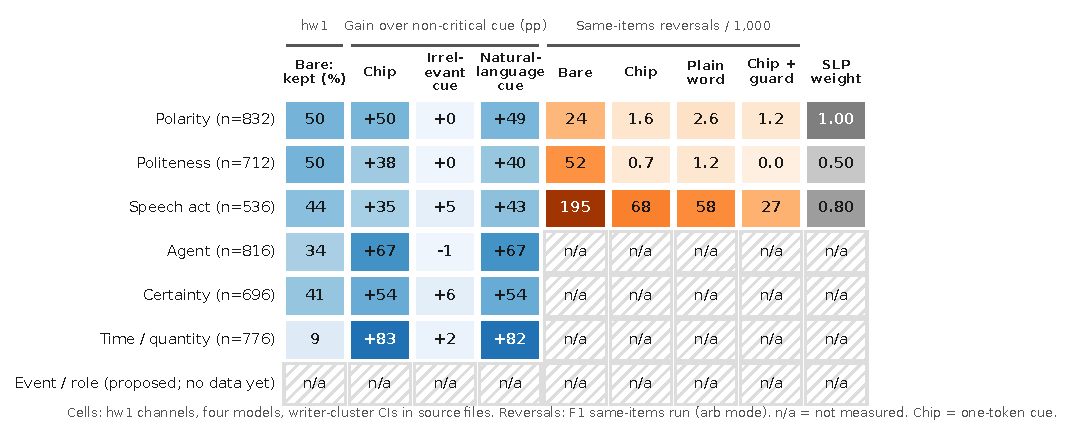
\includegraphics[width=\linewidth]{figs/fig4_dimension_table.pdf}
\caption{Dimension by intervention table. Left: share of bare outputs that keep the critical commitment (hw1, four models), and gain in that share over a non-critical cue for the chip, an irrelevant control cue and a natural-language cue. Right: same-items reversals per 1,000 messages for bare, chip, plain word and chip plus guard (\jmfOneUnits{} units; measured only for polarity, politeness and speech act), and the SLP severity weight (mean of two expert raters, $n=2$). Event/role structure is proposed but has no data. Every cell is printed; shading is redundant. Sources: \texttt{figs/figure\_values.json}.}\label{fig:table}
\Description{Dimension by intervention table.}
\end{figure}

\subsection{Cue Restoration Priced Per 1,000 Messages on the Same Items}\label{sec:price}

\paragraph{Design.}
The gains above come from constructed pairs. To price the cue on the messages that people actually shorten, we returned to the elicitation sample and took the \jmfOneUnits{} units whose source carried a cue that the human keywords dropped (polarity \jmfOneUnitsPol{}, politeness \jmfOneUnitsPolite{}, sentence type \jmfOneUnitsAct{}, the last a seeded subsample of question and request units). Each unit was regenerated by \jmfOneModels{} models (GPT-6.1-terra, Qwen2.5-7B, Llama-3.1-8B) under four arms at temperature zero: the stored bare output, the cue as a chip, the cue as a plain word, and the chip with the guard of \S\ref{sec:guard} monitoring the supplied chip. The restoration share is the proportion of units whose output honours the dropped cue; reversals per 1,000 messages are the exposure per 1,000 messages times one minus the restoration share. The bare arm reproduces the always-commit rates of \S\ref{sec:basecost}, so the unit construction matches. Disputed critical labels (\jmfOneArbRows{} rows) were resolved by the blind arbiter.

\paragraph{Results.}
Table~\ref{tab:price} gives the prices. Giving the cue on every message lowers polarity reversals from \jmfOneRevPolBare{} to \jmfOneRevPolChip{} (chip) or \jmfOneRevPolWord{} (word) per 1,000, and politeness reversals from \jmfOneRevPoliteBare{} to \jmfOneRevPoliteChip{} or \jmfOneRevPoliteWord{}. Chip and word are equivalent within 5 points on politeness (chip minus word \jmfOneChipMinusWordPolite{} points [\jmfOneChipMinusWordPoliteLo{}, \jmfOneChipMinusWordPoliteHi{}]) and not distinguishable on polarity (\jmfOneChipMinusWordPol{} [\jmfOneChipMinusWordPolLo{}, \jmfOneChipMinusWordPolHi{}]) or sentence type (\jmfOneChipMinusWordAct{} [\jmfOneChipMinusWordActLo{}, \jmfOneChipMinusWordActHi{}]). The guard on the chip arm helps on all three (polarity \jmfOneGuardGainPol{} points [\jmfOneGuardGainPolLo{}, \jmfOneGuardGainPolHi{}], politeness \jmfOneGuardGainPolite{} [\jmfOneGuardGainPoliteLo{}, \jmfOneGuardGainPoliteHi{}], sentence type \jmfOneGuardGainAct{} [\jmfOneGuardGainActLo{}, \jmfOneGuardGainActHi{}]); it raises the share of sentence-type units that honour the cue from \jmfOneRestActChip{}\% to \jmfOneRestActChipG{}\% [\jmfOneRestActChipGLo{}, \jmfOneRestActChipGHi{}]. Sentence type keeps the largest residual (\jmfOneRevActChipG{} [\jmfOneRevActChipGLo{}, \jmfOneRevActChipGHi{}] per 1,000 with chip and guard, from \jmfOneRevActBare{} bare), consistent with the speech-act dimension being the hardest in every earlier study.

\begin{table}[t]
\caption{Same-items price of the default and of cue restoration (\jmfOneUnits{} elicitation units, \jmfOneModels{} models, message-bootstrap 95\% intervals, arbiter-resolved labels). Each cell is the share of units whose output honours the dropped cue, followed by reversals per 1,000 messages if the arm is applied to every message and a cue is supplied each time. The price is the best case for the cue arms: it ignores the cost of cueing messages that need no cue and assumes the cue is elicited.}\label{tab:price}
\small
\begin{tabular}{lccccc}
\toprule
Dimension (units) & Quantity & Bare & Chip & Plain word & Chip + guard \\
\midrule
Polarity (\jmfOneUnitsPol{}) & Restored (\%) & \jmfOneRestPolBare{} & \jmfOneRestPolChip{} & \jmfOneRestPolWord{} & \jmfOneRestPolChipG{} \\
 & Reversals /1,000 & \jmfOneRevPolBare{} & \jmfOneRevPolChip{} [\jmfOneRevPolChipLo{}, \jmfOneRevPolChipHi{}] & \jmfOneRevPolWord{} [\jmfOneRevPolWordLo{}, \jmfOneRevPolWordHi{}] & \jmfOneRevPolChipG{} [\jmfOneRevPolChipGLo{}, \jmfOneRevPolChipGHi{}] \\
\addlinespace
Politeness (\jmfOneUnitsPolite{}) & Restored (\%) & \jmfOneRestPoliteBare{} & \jmfOneRestPoliteChip{} & \jmfOneRestPoliteWord{} & \jmfOneRestPoliteChipG{} \\
 & Reversals /1,000 & \jmfOneRevPoliteBare{} & \jmfOneRevPoliteChip{} [\jmfOneRevPoliteChipLo{}, \jmfOneRevPoliteChipHi{}] & \jmfOneRevPoliteWord{} [\jmfOneRevPoliteWordLo{}, \jmfOneRevPoliteWordHi{}] & \jmfOneRevPoliteChipG{} [\jmfOneRevPoliteChipGLo{}, \jmfOneRevPoliteChipGHi{}] \\
\addlinespace
Sentence type (\jmfOneUnitsAct{}) & Restored (\%) & \jmfOneRestActBare{} & \jmfOneRestActChip{} & \jmfOneRestActWord{} & \jmfOneRestActChipG{} \\
 & Reversals /1,000 & \jmfOneRevActBare{} & \jmfOneRevActChip{} [\jmfOneRevActChipLo{}, \jmfOneRevActChipHi{}] & \jmfOneRevActWord{} [\jmfOneRevActWordLo{}, \jmfOneRevActWordHi{}] & \jmfOneRevActChipG{} [\jmfOneRevActChipGLo{}, \jmfOneRevActChipGHi{}] \\
\bottomrule
\end{tabular}
\end{table}

\paragraph{A superseded estimate.}
An earlier version of this price transported the cue-honouring rate from the constructed pairs to the elicitation units. The measured rates do not match the transported ones for polarity or politeness (the transported rate was too optimistic for polarity and too pessimistic for politeness, in each case outside 5 points and outside the interval), so the measured rows replace the transported rows throughout.

\paragraph{Bound.}
Machine-judged outputs, three models, one prompt template, \jmfOneUnitsPol{} polarity units, and a price that assumes the cue is supplied. The restored outputs have no separate human check beyond the arbiter check (Section~\ref{sec:m-arbiter}).

% ------------------------------------------------------------------------------------------------
\subsection{Prior-Work Recap: The Commitment Guard}\label{sec:guard}

This subsection recaps the guard studies reported in our two earlier papers \cite{concurrent_se4all,concurrent_caleai}. It is subordinate to the writer-intent result: nothing in the argument of Section~\ref{sec:s4} depends on it, and the new material here is the human repair-usability audit (Section~\ref{sec:usability}) and the severity weighting (Section~\ref{sec:severity}).

\paragraph{Guard and baselines.}
The guard (G1) is a monitor on the output plus a bounded retry. The monitor flags an output that contradicts a supplied cue or that adds politeness the keywords do not carry; on a flag the model gets one short feedback turn that names the commitment it must keep, up to two retries at temperature zero, stopping at the first output the monitor does not flag. The monitor is a deterministic, rule-based extractor. A guard can look effective for a trivial reason, so we compare it with three alternatives that share the monitor, the trigger and the retry budget: a strip-only arm (G1s) that deletes an unsupplied ``please'' and makes no model call; a resample arm (G1r) that retries from the original prompt with no feedback at temperature $0.7$; and a feedback arm at temperature $0.7$ (G1t) that isolates feedback from decoding. The no-feedback baseline is G1r. The endpoint is a machine-scored partial predicate (the critical commitment and the absence of added politeness), not a usability judgement; usability is the subject of \S\ref{sec:usability}.

\paragraph{Transfer to fresh families (restated from our earlier papers).}
This result and the discovery-set guard result are reported in our earlier papers \cite{concurrent_se4all,concurrent_caleai}; we restate them here once, with the same frozen guard, because the audits below depend on them.
The frozen guard was applied, without change, to \jmgtFamilies{} fresh speech-act families that were not used to design it (\jmgtTargets{} target occurrences, \jmgwFlaggedF{} flagged requests). Joint pass rises from \jmgtJointP{}\% [\jmgtJointPLo{}, \jmgtJointPHi{}] to \jmgtJointG{}\% [\jmgtJointGLo{}, \jmgtJointGHi{}], a gain of \jmgwGain{} points [\jmgwGainLo{}, \jmgwGainHi{}]. Of the \jmgwStrictRepairN{} first-pass strict failures, \jmgwStrictRepairK{} (\jmgwStrictRepair{}\% [\jmgwStrictRepairLo{}, \jmgwStrictRepairHi{}]) are repaired; the guard rewrote \jmgwChangedK{} of \jmgwChangedN{} first-pass-correct targets and turned \jmgwPassToFailK{} passes into failures. The whole run took \jmgwGenCalls{} generation calls. On the discovery set the corresponding joint pass is \jmgbDiscPZero{}\% to \jmgbDiscGOne{}\% [\jmgbDiscGOneLo{}, \jmgbDiscGOneHi{}].

\paragraph{The no-feedback baseline.}
Table~\ref{tab:guard} compares the arms. Resampling without feedback gives about the strip-only gain on the fresh families (\jmgbWcGOner{}\% against \jmgbWcGOnes{}\%) and repairs \jmgbWcRepairGOner{}\% of strict failures against \jmgbWcRepairGOnes{}\% for the strip and \jmgbWcRepairGOne{}\% for the guard. The paired joint-pass contrast of the guard over the resample is \jmgbCWcGOneMGOner{} points [\jmgbCWcGOneMGOnerLo{}, \jmgbCWcGOneMGOnerHi{}] on the fresh families and \jmgbCDiscGOneMGOner{} [\jmgbCDiscGOneMGOnerLo{}, \jmgbCDiscGOneMGOnerHi{}] on the discovery set. Because the resample runs at temperature $0.7$ and the guard at zero, the clean contrast for the value of feedback is G1t minus G1r: \jmgbCWcGOnetMGOner{} points [\jmgbCWcGOnetMGOnerLo{}, \jmgbCWcGOnetMGOnerHi{}] on the fresh families and \jmgbCDiscGOnetMGOner{} [\jmgbCDiscGOnetMGOnerLo{}, \jmgbCDiscGOnetMGOnerHi{}] on discovery. Feedback adds value beyond resampling on both sets, and temperature is not what separates the guard from the baseline (G1 minus G1t: \jmgbCWcGOneMGOnet{} [\jmgbCWcGOneMGOnetLo{}, \jmgbCWcGOneMGOnetHi{}] on fresh families). The guard also beats the strip alone by \jmgwGOneMinusGOnes{} points [\jmgwGOneMinusGOnesLo{}, \jmgwGOneMinusGOnesHi{}], so the deletion explains part of the gain and not all of it.

\begin{table}[t]
\caption{The guard against its baselines (machine-scored joint pass, family-bootstrap 95\% intervals; strict repair is the share of first-pass strict failures repaired). Fresh families: \jmgbWcFamilies{} speech-act families, \jmgbWcTargets{} targets. Discovery: \jmgbDiscFamilies{} families, \jmgbDiscTargets{} targets. G1r is the no-feedback resample at temperature $0.7$.}\label{tab:guard}
\small
\begin{tabular}{lcccc}
\toprule
 & \multicolumn{2}{c}{Fresh families} & \multicolumn{2}{c}{Discovery} \\
\cmidrule(lr){2-3}\cmidrule(lr){4-5}
Arm & Joint pass (\%) & Strict repair & Joint pass (\%) & Strict repair \\
\midrule
First pass (P0) & \jmgbWcPZero{} [\jmgbWcPZeroLo{}, \jmgbWcPZeroHi{}] & --- & \jmgbDiscPZero{} [\jmgbDiscPZeroLo{}, \jmgbDiscPZeroHi{}] & --- \\
Strip only (G1s) & \jmgbWcGOnes{} [\jmgbWcGOnesLo{}, \jmgbWcGOnesHi{}] & \jmgbWcRepairGOnesK{}/\jmgbWcRepairGOnesN{} & \jmgbDiscGOnes{} [\jmgbDiscGOnesLo{}, \jmgbDiscGOnesHi{}] & \jmgbDiscRepairGOnesK{}/\jmgbDiscRepairGOnesN{} \\
Resample, no feedback (G1r) & \jmgbWcGOner{} [\jmgbWcGOnerLo{}, \jmgbWcGOnerHi{}] & \jmgbWcRepairGOnerK{}/\jmgbWcRepairGOnerN{} & \jmgbDiscGOner{} [\jmgbDiscGOnerLo{}, \jmgbDiscGOnerHi{}] & \jmgbDiscRepairGOnerK{}/\jmgbDiscRepairGOnerN{} \\
Feedback at $T=0.7$ (G1t) & \jmgbWcGOnet{} [\jmgbWcGOnetLo{}, \jmgbWcGOnetHi{}] & \jmgbWcRepairGOnetK{}/\jmgbWcRepairGOnetN{} & \jmgbDiscGOnet{} [\jmgbDiscGOnetLo{}, \jmgbDiscGOnetHi{}] & \jmgbDiscRepairGOnetK{}/\jmgbDiscRepairGOnetN{} \\
Guard (G1) & \jmgbWcGOne{} [\jmgbWcGOneLo{}, \jmgbWcGOneHi{}] & \jmgbWcRepairGOneK{}/\jmgbWcRepairGOneN{} & \jmgbDiscGOne{} [\jmgbDiscGOneLo{}, \jmgbDiscGOneHi{}] & \jmgbDiscRepairGOneK{}/\jmgbDiscRepairGOneN{} \\
\bottomrule
\end{tabular}
\end{table}

\paragraph{Bound.}
The endpoint is a machine-scored partial predicate on speech-act families; it supports the claim that the guard repairs commitment violations that a no-feedback retry does not, not a claim that its output is usable, fluent or preferred. Those questions are answered next, by people.

% ------------------------------------------------------------------------------------------------
\subsection{Repair Usability: A Blind Three-Rater Audit}\label{sec:usability}

\paragraph{Design.}
A guard that changes the text can make it worse to read. We audited this with a blind human audit under a decision rule frozen before any rating returned. The audit uses \jmpOneSevenItemsPerArm{} repaired texts and \jmpOneSevenItemsPerArm{} control texts (unrepaired outputs for which the monitor raised no flag, drawn from the same two pools), none of which had appeared in an earlier audit, rated by \jmpOneSevenRaters{} adult non-author classmates, \jmpOneSevenPerItem{} raters per item, with the arm hidden. The primary endpoint is the item-level majority of ``usable as the person's message''; secondary endpoints are meaning preserved against the keywords and cues and an invented stance or attitude. The frozen rule reads: if the interval for repaired minus control usable lies wholly below $-10$ points, the guard fails as a deployment clause; if it includes $-10$ but excludes zero, report a cost of uncertain size; if it includes zero, report no detectable cost. A comparison arm was added before any return to address the fact that controls never failed and repaired items did: the first-pass output that the guard replaced (\jmpOneSevenOrigItems{} items, each paired with its repair).

\paragraph{Result under the frozen rule.}
Repaired texts were usable in \jmpOneSevenRepUsableK{} of \jmpOneSevenRepUsableN{} items (\jmpOneSevenRepUsable{}\% [\jmpOneSevenRepUsableLo{}, \jmpOneSevenRepUsableHi{}]) and control texts in \jmpOneSevenCtlUsableK{} of \jmpOneSevenCtlUsableN{} (\jmpOneSevenCtlUsable{}\% [\jmpOneSevenCtlUsableLo{}, \jmpOneSevenCtlUsableHi{}]). The difference is \jmpOneSevenDiffUsable{} points [\jmpOneSevenDiffUsableLo{}, \jmpOneSevenDiffUsableHi{}]. The interval includes zero, so under the frozen rule the audit detects no usability cost, but the interval extends to \jmpOneSevenDiffUsableLo{} points: the audit is inconclusive, it neither shows nor excludes a cost, and it does not establish equivalence. Table~\ref{tab:p17} gives the endpoints. Repaired texts preserved the meaning less often than controls (\jmpOneSevenDiffPres{} points [\jmpOneSevenDiffPresLo{}, \jmpOneSevenDiffPresHi{}]) and so did the combined endpoint, usable and preserving (\jmpOneSevenDiffUsPres{} [\jmpOneSevenDiffUsPresLo{}, \jmpOneSevenDiffUsPresHi{}]); invented stance did not differ (\jmpOneSevenDiffStance{} [\jmpOneSevenDiffStanceLo{}, \jmpOneSevenDiffStanceHi{}]). The comparison is between inputs the first pass got wrong and inputs it got right, so the gap partly measures item difficulty and not the repair; the comparison against each repair's own failed original, below, holds the item fixed.

\begin{table}[t]
\caption{Blind audit of guard repairs (the repair-usability audit; \jmpOneSevenRaters{} raters, \jmpOneSevenPerItem{} per item, item-level strict majority; Wilson 95\% intervals for rates, Newcombe 95\% intervals for differences; preserving and stance exclude one item with no majority). The items are a pre-specified deterministic list, not a probability sample, so the rates describe these items.}\label{tab:p17}
\small
\begin{tabular}{lccc}
\toprule
Endpoint & Repaired & Control & Repaired $-$ control (points) \\
\midrule
Usable (primary) & \jmpOneSevenRepUsableK{}/\jmpOneSevenRepUsableN{} = \jmpOneSevenRepUsable{}\% [\jmpOneSevenRepUsableLo{}, \jmpOneSevenRepUsableHi{}] & \jmpOneSevenCtlUsableK{}/\jmpOneSevenCtlUsableN{} = \jmpOneSevenCtlUsable{}\% [\jmpOneSevenCtlUsableLo{}, \jmpOneSevenCtlUsableHi{}] & \jmpOneSevenDiffUsable{} [\jmpOneSevenDiffUsableLo{}, \jmpOneSevenDiffUsableHi{}] \\
Meaning preserved & \jmpOneSevenRepPresK{}/\jmpOneSevenRepPresN{} = \jmpOneSevenRepPres{}\% [\jmpOneSevenRepPresLo{}, \jmpOneSevenRepPresHi{}] & \jmpOneSevenCtlPresK{}/\jmpOneSevenCtlPresN{} = \jmpOneSevenCtlPres{}\% [\jmpOneSevenCtlPresLo{}, \jmpOneSevenCtlPresHi{}] & \jmpOneSevenDiffPres{} [\jmpOneSevenDiffPresLo{}, \jmpOneSevenDiffPresHi{}] \\
Invented stance & \jmpOneSevenRepStanceK{}/\jmpOneSevenRepStanceN{} = \jmpOneSevenRepStance{}\% [\jmpOneSevenRepStanceLo{}, \jmpOneSevenRepStanceHi{}] & \jmpOneSevenCtlStanceK{}/\jmpOneSevenCtlStanceN{} = \jmpOneSevenCtlStance{}\% [\jmpOneSevenCtlStanceLo{}, \jmpOneSevenCtlStanceHi{}] & \jmpOneSevenDiffStance{} [\jmpOneSevenDiffStanceLo{}, \jmpOneSevenDiffStanceHi{}] \\
\bottomrule
\end{tabular}
\end{table}

\paragraph{Against each repair's own failed original.}
Paired with the first-pass output that the guard replaced, repairs preserve the meaning more often (\jmpOneSevenOrigPres{} points [\jmpOneSevenOrigPresLo{}, \jmpOneSevenOrigPresHi{}], $p=\jmpOneSevenOrigPresP{}$ on \jmpOneSevenOrigPresPairs{} pairs) and invent a stance less often (\jmpOneSevenOrigStance{} points [\jmpOneSevenOrigStanceLo{}, \jmpOneSevenOrigStanceHi{}], $p=\jmpOneSevenOrigStanceP{}$ on \jmpOneSevenOrigStancePairs{} pairs). Usability shows no detectable change (\jmpOneSevenOrigUsable{} points [\jmpOneSevenOrigUsableLo{}, \jmpOneSevenOrigUsableHi{}], $p=\jmpOneSevenOrigUsableP{}$). Relative to the failed original, the repair preserves the meaning and removes the invented stance without a detectable change in how usable the sentence is.

\paragraph{Heterogeneity.}
Usability varies by the model that produced the repair. Gemma-3-4B repairs are usable in \jmpOneSevenRepGemmaUsableK{} of \jmpOneSevenRepGemmaUsableN{} (\jmpOneSevenRepGemmaUsable{}\%), against \jmpOneSevenRepLlamaUsableK{} of \jmpOneSevenRepLlamaUsableN{} for Llama-3.1-8B, \jmpOneSevenRepQwenSUsableK{} of \jmpOneSevenRepQwenSUsableN{} for Qwen2.5-7B and \jmpOneSevenRepTerraUsableK{} of \jmpOneSevenRepTerraUsableN{} for GPT-6.1-terra. These are descriptive counts on an unbalanced list. They suggest that a repair is only as readable as the repairing model's prose, which the pooled estimate hides.

\paragraph{Bound.}
\jmpOneSevenItemsPerArm{} items per arm from a fixed list, classmate raters rather than AAC users or clinicians, and a rule that detects no cost without excluding a cost of up to \jmpOneSevenDiffUsableLo{} points.

% ------------------------------------------------------------------------------------------------
\subsection{Weighting the Failures by Clinical Severity}\label{sec:severity}

Two speech-language pathologists, anonymous and paid as expert annotators of study materials, rated how serious each kind of silent meaning change would be if spoken as a client's message, and then rated stored outputs with the arm hidden: guard repairs (\jmslpAccRepairN{} ratings), the matching first-pass originals (\jmslpAccOrigN{}), chip outputs (\jmslpAccChipN{}) and plain-word outputs (\jmslpAccWordN{}); a rating is one rater's judgement of one output. This is an expert review with $n=2$ raters, not a population estimate, and the agreement statistics describe these two raters. Both rated negation dropped or added as the most serious change (\jmslpNegSeverity{} of 5) and both would block it (\jmslpNegBlock{}\%).

We weight each judge-flagged failure by the severity of its type, taking the largest weight on an output. On the fresh speech-act families the guard lowers the weighted failure rate from \jmslpWGuardBase{}\% to \jmslpWGuardG{}\% (strip only: \jmslpWGuardGs{}\%; unweighted \jmslpUGuardBase{}\% to \jmslpUGuardG{}\%; \jmslpWcN{} targets). On the human-written pairs the weighted failure rate is \jmslpWCueBare{}\% for bare keywords, \jmslpWCueChip{}\% with a chip and \jmslpWCueWord{}\% with a plain word, against \jmslpWCueIrrel{}\% with an irrelevant chip (\jmslpHwN{} rows per arm). The bare and irrelevant rates are inflated by the pair design, because two variants share one bare input; the comparison of interest is chip against word against the irrelevant control, and it again shows that the cue content carries the effect.

Rated directly, the SLPs judged the guard's repairs acceptable to speak as they stand in \jmslpAccRepair{}\% of ratings, and as they stand or after a small edit in \jmslpRepairEdit{}\%, against \jmslpAccOrig{}\% as they stand for the matching originals. Chip outputs were acceptable as they stand in \jmslpAccChip{}\% of ratings and plain-word outputs in \jmslpAccWord{}\%. The two raters agreed on whether an output says what the selected words mean on \jmslpAgreeA{}\% of items ($\kappa=\jmslpKappaA{}$) and on whether it is acceptable to speak on \jmslpAgreeB{}\% ($\kappa=\jmslpKappaB{}$); we report these as descriptions of this pair. The arms were rated on different numbers of items, so the acceptability figures are descriptive and do not rank the arms.

% ------------------------------------------------------------------------------------------------
\subsection{What These Studies Establish}\label{sec:establish}

The default is measurable, mostly attributable to a missing cue, and a supplied cue removes most of it on the dimensions measured. Against people's own keyword choices the affirmative default is the right guess for negation and costs about \jmtTwoRevPol{} silent reversals per 1,000 messages; it is not a prompt artefact and holds in \jmbreadthModels{} models from \jmbreadthFamilies{} families; a one-token cue or a plain word removes nearly all of the negation and politeness cost on the same items (to \jmfOneRevPolChip{} and \jmfOneRevPoliteChip{} per 1,000 with a chip); the cue's content, not its presence, does the work; and the guard (recapped in Section~\ref{sec:guard}) repairs violations that a no-feedback retry does not, and the blind repair audit could not exclude a usability cost (Section~\ref{sec:usability}). These results answer whether a commitment is preserved. Whether the preserved draft is the message the writer meant is a different question, which \S\ref{sec:waterfall} takes up with the writers themselves.
.
% Every number is a \jm... macro from make_macros.py (function s3() and earlier functions); no hand-typed numbers.
% Examples are stored outputs chosen by a declared rule (analysis/hw1/examples.md). Citations are limited to
% records already in refs.bib; nothing new was opened for this section.
% Labels defined here: sec:default (section), sec:basecost, sec:robust, sec:cue, sec:price, sec:asks, sec:guard, sec:usability, sec:severity.
% Needs \usepackage{booktabs} (acmart loads it).

\section{Studies and Results I: Defaults, Cue Restoration and the Guard}\label{sec:default}

This section reports the studies that establish what the default costs and what repairs it. Each study states its population, its estimator and its denominator, and each result is bounded once, where it is reported. We begin with the cost of the default measured against what people actually type (\S\ref{sec:basecost}), test whether the default belongs to the prompt or to the models (\S\ref{sec:robust}), show that a cue restores the commitment and that the cue's content is what does it (\S\ref{sec:cue}), price the restoration per 1,000 messages on the same items (\S\ref{sec:price}), ask whether any rule for when to ask beats chance (\S\ref{sec:asks}), and then evaluate the guard against a no-feedback baseline (\S\ref{sec:guard}), a blind human audit of its repairs (\S\ref{sec:usability}) and expert severity weights (\S\ref{sec:severity}).

\paragraph{Conventions common to all studies.}
Model outputs are labelled by two machine judges (J1, J2); disagreements on the critical commitment go to a blind arbiter that sees only the output text, and no label falls back to J1 when the arbiter is missing. Intervals are 95\% percentile bootstrap intervals clustered by writer (human-written pairs), by family (machine-written families and the guard) or by message (the elicitation sample). The human-written, legend, control and guard analyses use \jmconvBoot{} resamples with seed \jmconvSeed{}, the same-items study uses \jmconvBootFOne{} resamples with seed \jmconvSeedFOne{}, and the elicitation-sample prices and ask-policy contrasts use the resample counts stated in their reports. Rates ``per 1,000 messages'' are rates over the sampled units, not deployment rates. Where a decision rule governs a verdict (the legend test, the same-items comparisons, the guard baseline and the usability audit), it was written down and git-timestamped before the outcomes it governs were generated or returned; we do not call any of the studies pre-registered. Machine labels are used throughout this section; where a human check of the machine labels exists it is reported in the study that uses the labels, and the checks that have not yet returned are named as such.

% ------------------------------------------------------------------------------------------------
\subsection{What the Default Costs, Priced Against Human Base Rates}\label{sec:basecost}

\paragraph{Setting.}
A keyword string that omits a cue leaves the model to choose a reading, and the choice is a default. Whether a default is a good guess depends on how often the omitted cue was present in what the writer meant. We measured that base rate from people. The elicitation sample consists of \jmtTwoMessages{} source messages from an AAC-style corpus (\jmtTwoCorpus{} messages in total, of which \jmtTwoCorpusNeg{}\% are negated by a detector label), each shortened to keywords by three human keyword sets, giving \jmtTwoUnits{} keyword units. Stored outputs of \jmbreadthOrigModels{} generators were scored for three commitment dimensions (negation, politeness, sentence type), the dimensions for which a lexical test of ``the keywords carry the cue'' exists. The source cue labels are detector labels; these labels have no human check, so the prices below carry the detector's error and are provisional.

\paragraph{Affirmative is the right guess for negation; the cost is the asymmetry.}
Among keyword strings with no negation word, the source was negated in \jmtTwoPostPol{}\% [\jmtTwoPostPolLo{}, \jmtTwoPostPolHi{}] of cases (\jmtTwoPostBayesPol{}\% by Bayes' rule with the corpus prevalence; \jmtTwoPolRandHalf{}\% in the unweighted random half). Guessing the affirmative reading is therefore correct for all but a few messages in a hundred, and the models take it: they output an affirmative sentence for \jmtTwoAffGivenNoNeg{}\% of such inputs. The direction of the default is the rational one, which is consistent with prior reports that language models state negative content too positively \cite{chen2023say}; we do not present the default as new. What the base rate adds is the price. People dropped the negation word from \jmtTwoDroppedPol{}\% [\jmtTwoDroppedPolLo{}, \jmtTwoDroppedPolHi{}] of the negated messages, so an affirmative sentence silently reverses \jmtTwoRevPol{} [\jmtTwoRevPolLo{}, \jmtTwoRevPolHi{}] messages per 1,000, while a spurious negation is introduced in \jmtTwoSpurPol{} per 1,000. The affirmative guess breaks even with the opposite guess only if a reversed negation costs less than \jmtTwoBreakPol{} times a spurious one, and a prompt would have to be shown on about \jmtTwoQueriesPol{} inputs per reversal it prevents. The models' confidence also exceeds the evidence: they assert a negation on \jmtTwoModelCuePol{}\% of these inputs where the base rate is \jmtTwoPostPol{}\%.

\paragraph{Politeness and sentence type differ in kind.}
For politeness the default is calibrated: the source was polite in \jmtTwoPostPolite{}\% [\jmtTwoPostPoliteLo{}, \jmtTwoPostPoliteHi{}] of unmarked inputs and models add politeness to \jmtTwoModelCuePolite{}\%. Politeness the writer typed is lost for \jmtTwoRevPolite{} messages per 1,000, with a break-even ratio of \jmtTwoBreakPolite{}, so the asymmetry is milder than for negation; the opposite error, politeness added to a plain message, occurs in \jmtTwoSpurPolite{} per 1,000. For sentence type the statement default is not the Bayes-preferred guess at all: the source was a question, request or other non-statement in \jmtTwoPostAct{}\% [\jmtTwoPostActLo{}, \jmtTwoPostActHi{}] of unmarked inputs, while models assert one on only \jmtTwoModelCueAct{}\%, and \jmtTwoRevAct{} [\jmtTwoRevActLo{}, \jmtTwoRevActHi{}] messages per 1,000 have their sentence type reversed or flattened (break-even ratio \jmtTwoBreakAct{}: the statement default pays only if the two errors cost about the same).
Table~\ref{tab:basecost} collects these rows.

\begin{table}[t]
\caption{The default priced against human base rates (elicitation sample, \jmtTwoUnits{} keyword units from \jmtTwoMessages{} messages; Horvitz--Thompson weights; message-bootstrap 95\% intervals). Prior is the share of keyword strings without the cue whose source message carried it; model asserts cue is the share of such inputs for which the model's output asserts the cue-bearing value. Reversals are messages whose source has the cue, whose keywords lack it and whose output lacks it; the opposite error is an output that asserts the cue when the source lacks it; break-even is the cost ratio of a reversal to an opposite error at which the default stops paying. Source labels are detector labels.}\label{tab:basecost}
\footnotesize
\begin{tabular}{@{}lccccc@{}}
\toprule
Dimension & Prior [95\% CI] & Model asserts cue & Reversals /1,000 [CI] & Opposite /1,000 & Break-even \\
\midrule
Negation (affirmative default) & \jmtTwoPostPol{}\% [\jmtTwoPostPolLo{}, \jmtTwoPostPolHi{}] & \jmtTwoModelCuePol{}\% & \jmtTwoRevPol{} [\jmtTwoRevPolLo{}, \jmtTwoRevPolHi{}] & \jmtTwoSpurPol{} & \jmtTwoBreakPol{} \\
Politeness (plain default) & \jmtTwoPostPolite{}\% [\jmtTwoPostPoliteLo{}, \jmtTwoPostPoliteHi{}] & \jmtTwoModelCuePolite{}\% & \jmtTwoRevPolite{} [\jmtTwoRevPoliteLo{}, \jmtTwoRevPoliteHi{}] & \jmtTwoSpurPolite{} & \jmtTwoBreakPolite{} \\
Sentence type (statement default) & \jmtTwoPostAct{}\% [\jmtTwoPostActLo{}, \jmtTwoPostActHi{}] & \jmtTwoModelCueAct{}\% & \jmtTwoRevAct{} [\jmtTwoRevActLo{}, \jmtTwoRevActHi{}] & \jmtTwoSpurAct{} & \jmtTwoBreakAct{} \\
\bottomrule
\end{tabular}
\end{table}

\paragraph{The same default in human-written pairs.}
The human-written pairs (\S\ref{sec:cue}) test the default where the truth is known. Each pair differs in one commitment and shares one bare input, so a model that commits to one reading is wrong on exactly one variant and the true affirmative rate is 50\%. On the bare channel the models chose the affirmative reading in \jmtTwoHwAffShare{}\% of valid outputs.

\paragraph{Bound.}
Source cue labels are detector labels, the sentence-type ``no cue'' condition is a lexical proxy, the frame prevalence of negation (\jmtTwoPrevPol{}\%) exceeds the corpus value, and the prices are rates over a sampled elicitation frame. We therefore read the table as the cost structure of the default, not as a deployment rate.

% ------------------------------------------------------------------------------------------------
\paragraph{Appendix material.} The model-breadth tables and legend test (Appendix~\ref{sec:robust}) and the ask-policy arithmetic (Appendix~\ref{sec:asks}) are in the appendix; the main text uses only their headline results.

\subsection{A Cue Restores the Commitment, and the Content of the Cue Does It}\label{sec:cue}

\paragraph{Human-written pairs.}
To move beyond machine-written test items, \jmhwWritersTotal{} adult non-author classmates wrote sentence pairs that differ in one commitment and chose their own keywords; pairs were kept only after classmate checks, and \jmhwFamilies{} families were analysed, with \jmhwChipGainWriters{} to \jmhwAffShareWriters{} writers contributing to each contrast. Each family was expanded by \jmbreadthOrigModels{} models under bare keywords, a non-critical extra keyword, the cue as a one-token chip (for example \texttt{[NOT]}), the full cue set, and the full original text. The primary contrasts are those of the machine-written confirmation set (Holm-corrected over three); the human-written pairs are an exploratory replication of them. The chip gain over a non-critical word on speech act is \jmhwChipGain{} points [\jmhwChipGainLo{}, \jmhwChipGainHi{}] (\jmhwChipGainWriters{} writers, \jmhwChipGainFamilies{} families). When the full sentence is given, politeness is added to plain messages more often than it is removed from polite ones, by \jmhwPolGain{} points [\jmhwPolGainLo{}, \jmhwPolGainHi{}]. The bare affirmative share (\jmhwAffAll{}\%, \S\ref{sec:basecost}) is the third contrast. All three agree in direction and in decision with the machine-written confirmation set. Because each contrast rests on a handful of writers, we claim the direction and its consistency across writers and models, not the width of the intervals.

\paragraph{One stored case, by declared rule.}
The rule: order the analysed polarity families by the SHA-256 of the family identifier and take the first one in which a bare output commits to the wrong value while the chip output matches. That family is \texttt{hw-pol-075}, the model is Gemma-3-4B, and the target is the negated reading of ``The supervisor does not read my schedule.''

\begin{center}\small
\begin{tabular}{lll}
\toprule
Channel & Input & Stored output \\
\midrule
bare & \texttt{supervisor read} & ``The supervisor read.'' (affirmative) \\
chip & \texttt{[NOT] supervisor read} & ``The supervisor did not read.'' (negated) \\
\bottomrule
\end{tabular}
\end{center}

\noindent
In this dimension a bare output commits to the wrong value in \jmexPolBareWrong{}\% [\jmexPolBareWrongLo{}, \jmexPolBareWrongHi{}] of bare rows (the design ceiling), and when it does the chip output matches the target in \jmexPolRepair{}\% [\jmexPolRepairLo{}, \jmexPolRepairHi{}] of \jmexPolRepairN{} such rows. The same rule applied to speech act selects a family whose chip outputs match the target in a smaller share, \jmexActRepair{}\% [\jmexActRepairLo{}, \jmexActRepairHi{}] of \jmexActRepairN{} rows, in line with the larger residual for sentence type in \S\ref{sec:price}.

\paragraph{Six dimensions.}
Table~\ref{tab:sixdim} reports the cue gain for every measured dimension with its two controls. An irrelevant chip (a cue from another dimension, with the same token cost) adds about nothing on polarity, politeness, agent and time (at most \jmctlIrrelAddTime{} points) and a small amount on certainty (\jmctlIrrelAddCert{} [\jmctlIrrelAddCertLo{}, \jmctlIrrelAddCertHi{}]) and speech act (\jmctlIrrelAddAct{} [\jmctlIrrelAddActLo{}, \jmctlIrrelAddActHi{}]). The relevant chip beats the irrelevant chip by \jmctlOverIrrelAct{} to \jmctlOverIrrelTime{} points, so the gain is the content of the cue and not the presence of an extra token. A plain-language word delivers the same restoration as the chip within 5 points on every dimension except speech act; on speech act the word is better than the chip (chip minus word \jmctlOverWordAct{} points [\jmctlOverWordActLo{}, \jmctlOverWordActHi{}]). We do not claim that the chip is better than a plain word.

\begin{table}[t]
\caption{Cue restoration and its controls in human-written pairs (critical-commitment match, pooled over four models, writer-cluster 95\% intervals; points). Chip gain is chip minus non-critical word. Polarity and politeness bare matches sit at 50\% by design because both variants share one bare input; their informative quantity is the gain. Full input is the whole original sentence.}\label{tab:sixdim}
\small
\begin{tabular}{lccccc}
\toprule
Dimension & Bare match (\%) & Chip match (\%) & Chip gain [CI] & Irrelevant chip adds [CI] & Chip $-$ word [CI] \\
\midrule
Agent & \jmhwMatchBareAgent{} & \jmhwMatchChipAgent{} & \jmctlGAgent{} [\jmctlGAgentLo{}, \jmctlGAgentHi{}] & \jmctlIrrelAddAgent{} [\jmctlIrrelAddAgentLo{}, \jmctlIrrelAddAgentHi{}] & \jmctlOverWordAgent{} [\jmctlOverWordAgentLo{}, \jmctlOverWordAgentHi{}] \\
Time / quantity & \jmhwMatchBareTime{} & \jmhwMatchChipTime{} & \jmctlGTime{} [\jmctlGTimeLo{}, \jmctlGTimeHi{}] & \jmctlIrrelAddTime{} [\jmctlIrrelAddTimeLo{}, \jmctlIrrelAddTimeHi{}] & \jmctlOverWordTime{} [\jmctlOverWordTimeLo{}, \jmctlOverWordTimeHi{}] \\
Certainty & \jmhwMatchBareCert{} & \jmhwMatchChipCert{} & \jmctlGCert{} [\jmctlGCertLo{}, \jmctlGCertHi{}] & \jmctlIrrelAddCert{} [\jmctlIrrelAddCertLo{}, \jmctlIrrelAddCertHi{}] & \jmctlOverWordCert{} [\jmctlOverWordCertLo{}, \jmctlOverWordCertHi{}] \\
Polarity & \jmhwMatchBarePol{} & \jmhwMatchChipPol{} & \jmctlGPol{} [\jmctlGPolLo{}, \jmctlGPolHi{}] & \jmctlIrrelAddPol{} [\jmctlIrrelAddPolLo{}, \jmctlIrrelAddPolHi{}] & \jmctlOverWordPol{} [\jmctlOverWordPolLo{}, \jmctlOverWordPolHi{}] \\
Politeness & \jmhwMatchBarePolite{} & \jmhwMatchChipPolite{} & \jmctlGPolite{} [\jmctlGPoliteLo{}, \jmctlGPoliteHi{}] & \jmctlIrrelAddPolite{} [\jmctlIrrelAddPoliteLo{}, \jmctlIrrelAddPoliteHi{}] & \jmctlOverWordPolite{} [\jmctlOverWordPoliteLo{}, \jmctlOverWordPoliteHi{}] \\
Speech act & \jmhwMatchBareAct{} & \jmhwMatchChipAct{} & \jmctlGAct{} [\jmctlGActLo{}, \jmctlGActHi{}] & \jmctlIrrelAddAct{} [\jmctlIrrelAddActLo{}, \jmctlIrrelAddActHi{}] & \jmctlOverWordAct{} [\jmctlOverWordActLo{}, \jmctlOverWordActHi{}] \\
\bottomrule
\end{tabular}
\end{table}

\paragraph{Bound.}
\jmhwChipGainWriters{} to \jmhwAffShareWriters{} writers per dimension, one prompt template, and machine labels (with a blind arbiter for disputes); treated outputs have no separate human check beyond the arbiter check (Section~\ref{sec:m-arbiter}).

% ------------------------------------------------------------------------------------------------

\begin{figure}[t]
\centering
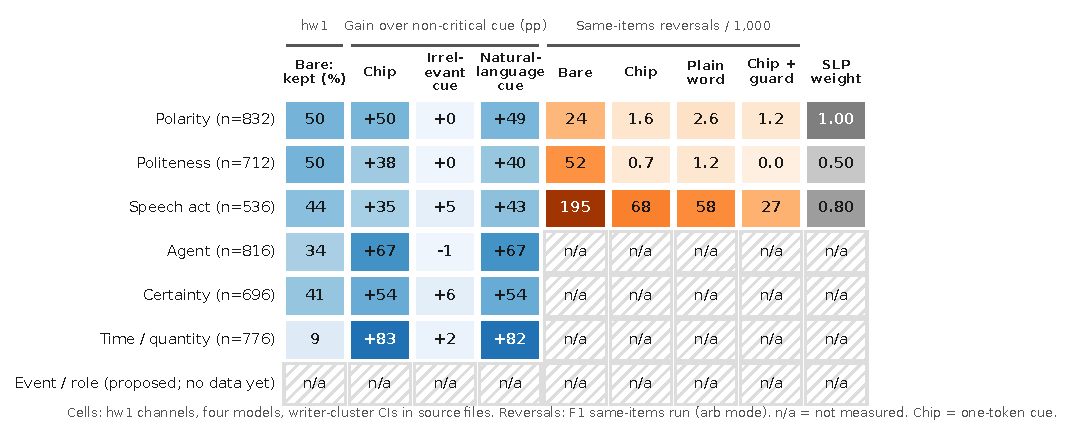
\includegraphics[width=\linewidth]{figs/fig4_dimension_table.pdf}
\caption{Dimension by intervention table. Left: share of bare outputs that keep the critical commitment (hw1, four models), and gain in that share over a non-critical cue for the chip, an irrelevant control cue and a natural-language cue. Right: same-items reversals per 1,000 messages for bare, chip, plain word and chip plus guard (\jmfOneUnits{} units; measured only for polarity, politeness and speech act), and the SLP severity weight (mean of two expert raters, $n=2$). Event/role structure is proposed but has no data. Every cell is printed; shading is redundant. Sources: \texttt{figs/figure\_values.json}.}\label{fig:table}
\Description{Dimension by intervention table.}
\end{figure}

\subsection{Cue Restoration Priced Per 1,000 Messages on the Same Items}\label{sec:price}

\paragraph{Design.}
The gains above come from constructed pairs. To price the cue on the messages that people actually shorten, we returned to the elicitation sample and took the \jmfOneUnits{} units whose source carried a cue that the human keywords dropped (polarity \jmfOneUnitsPol{}, politeness \jmfOneUnitsPolite{}, sentence type \jmfOneUnitsAct{}, the last a seeded subsample of question and request units). Each unit was regenerated by \jmfOneModels{} models (GPT-6.1-terra, Qwen2.5-7B, Llama-3.1-8B) under four arms at temperature zero: the stored bare output, the cue as a chip, the cue as a plain word, and the chip with the guard of \S\ref{sec:guard} monitoring the supplied chip. The restoration share is the proportion of units whose output honours the dropped cue; reversals per 1,000 messages are the exposure per 1,000 messages times one minus the restoration share. The bare arm reproduces the always-commit rates of \S\ref{sec:basecost}, so the unit construction matches. Disputed critical labels (\jmfOneArbRows{} rows) were resolved by the blind arbiter.

\paragraph{Results.}
Table~\ref{tab:price} gives the prices. Giving the cue on every message lowers polarity reversals from \jmfOneRevPolBare{} to \jmfOneRevPolChip{} (chip) or \jmfOneRevPolWord{} (word) per 1,000, and politeness reversals from \jmfOneRevPoliteBare{} to \jmfOneRevPoliteChip{} or \jmfOneRevPoliteWord{}. Chip and word are equivalent within 5 points on politeness (chip minus word \jmfOneChipMinusWordPolite{} points [\jmfOneChipMinusWordPoliteLo{}, \jmfOneChipMinusWordPoliteHi{}]) and not distinguishable on polarity (\jmfOneChipMinusWordPol{} [\jmfOneChipMinusWordPolLo{}, \jmfOneChipMinusWordPolHi{}]) or sentence type (\jmfOneChipMinusWordAct{} [\jmfOneChipMinusWordActLo{}, \jmfOneChipMinusWordActHi{}]). The guard on the chip arm helps on all three (polarity \jmfOneGuardGainPol{} points [\jmfOneGuardGainPolLo{}, \jmfOneGuardGainPolHi{}], politeness \jmfOneGuardGainPolite{} [\jmfOneGuardGainPoliteLo{}, \jmfOneGuardGainPoliteHi{}], sentence type \jmfOneGuardGainAct{} [\jmfOneGuardGainActLo{}, \jmfOneGuardGainActHi{}]); it raises the share of sentence-type units that honour the cue from \jmfOneRestActChip{}\% to \jmfOneRestActChipG{}\% [\jmfOneRestActChipGLo{}, \jmfOneRestActChipGHi{}]. Sentence type keeps the largest residual (\jmfOneRevActChipG{} [\jmfOneRevActChipGLo{}, \jmfOneRevActChipGHi{}] per 1,000 with chip and guard, from \jmfOneRevActBare{} bare), consistent with the speech-act dimension being the hardest in every earlier study.

\begin{table}[t]
\caption{Same-items price of the default and of cue restoration (\jmfOneUnits{} elicitation units, \jmfOneModels{} models, message-bootstrap 95\% intervals, arbiter-resolved labels). Each cell is the share of units whose output honours the dropped cue, followed by reversals per 1,000 messages if the arm is applied to every message and a cue is supplied each time. The price is the best case for the cue arms: it ignores the cost of cueing messages that need no cue and assumes the cue is elicited.}\label{tab:price}
\small
\begin{tabular}{lccccc}
\toprule
Dimension (units) & Quantity & Bare & Chip & Plain word & Chip + guard \\
\midrule
Polarity (\jmfOneUnitsPol{}) & Restored (\%) & \jmfOneRestPolBare{} & \jmfOneRestPolChip{} & \jmfOneRestPolWord{} & \jmfOneRestPolChipG{} \\
 & Reversals /1,000 & \jmfOneRevPolBare{} & \jmfOneRevPolChip{} [\jmfOneRevPolChipLo{}, \jmfOneRevPolChipHi{}] & \jmfOneRevPolWord{} [\jmfOneRevPolWordLo{}, \jmfOneRevPolWordHi{}] & \jmfOneRevPolChipG{} [\jmfOneRevPolChipGLo{}, \jmfOneRevPolChipGHi{}] \\
\addlinespace
Politeness (\jmfOneUnitsPolite{}) & Restored (\%) & \jmfOneRestPoliteBare{} & \jmfOneRestPoliteChip{} & \jmfOneRestPoliteWord{} & \jmfOneRestPoliteChipG{} \\
 & Reversals /1,000 & \jmfOneRevPoliteBare{} & \jmfOneRevPoliteChip{} [\jmfOneRevPoliteChipLo{}, \jmfOneRevPoliteChipHi{}] & \jmfOneRevPoliteWord{} [\jmfOneRevPoliteWordLo{}, \jmfOneRevPoliteWordHi{}] & \jmfOneRevPoliteChipG{} [\jmfOneRevPoliteChipGLo{}, \jmfOneRevPoliteChipGHi{}] \\
\addlinespace
Sentence type (\jmfOneUnitsAct{}) & Restored (\%) & \jmfOneRestActBare{} & \jmfOneRestActChip{} & \jmfOneRestActWord{} & \jmfOneRestActChipG{} \\
 & Reversals /1,000 & \jmfOneRevActBare{} & \jmfOneRevActChip{} [\jmfOneRevActChipLo{}, \jmfOneRevActChipHi{}] & \jmfOneRevActWord{} [\jmfOneRevActWordLo{}, \jmfOneRevActWordHi{}] & \jmfOneRevActChipG{} [\jmfOneRevActChipGLo{}, \jmfOneRevActChipGHi{}] \\
\bottomrule
\end{tabular}
\end{table}

\paragraph{A superseded estimate.}
An earlier version of this price transported the cue-honouring rate from the constructed pairs to the elicitation units. The measured rates do not match the transported ones for polarity or politeness (the transported rate was too optimistic for polarity and too pessimistic for politeness, in each case outside 5 points and outside the interval), so the measured rows replace the transported rows throughout.

\paragraph{Bound.}
Machine-judged outputs, three models, one prompt template, \jmfOneUnitsPol{} polarity units, and a price that assumes the cue is supplied. The restored outputs have no separate human check beyond the arbiter check (Section~\ref{sec:m-arbiter}).

% ------------------------------------------------------------------------------------------------
\subsection{Prior-Work Recap: The Commitment Guard}\label{sec:guard}

This subsection recaps the guard studies reported in our two earlier papers \cite{concurrent_se4all,concurrent_caleai}. It is subordinate to the writer-intent result: nothing in the argument of Section~\ref{sec:s4} depends on it, and the new material here is the human repair-usability audit (Section~\ref{sec:usability}) and the severity weighting (Section~\ref{sec:severity}).

\paragraph{Guard and baselines.}
The guard (G1) is a monitor on the output plus a bounded retry. The monitor flags an output that contradicts a supplied cue or that adds politeness the keywords do not carry; on a flag the model gets one short feedback turn that names the commitment it must keep, up to two retries at temperature zero, stopping at the first output the monitor does not flag. The monitor is a deterministic, rule-based extractor. A guard can look effective for a trivial reason, so we compare it with three alternatives that share the monitor, the trigger and the retry budget: a strip-only arm (G1s) that deletes an unsupplied ``please'' and makes no model call; a resample arm (G1r) that retries from the original prompt with no feedback at temperature $0.7$; and a feedback arm at temperature $0.7$ (G1t) that isolates feedback from decoding. The no-feedback baseline is G1r. The endpoint is a machine-scored partial predicate (the critical commitment and the absence of added politeness), not a usability judgement; usability is the subject of \S\ref{sec:usability}.

\paragraph{Transfer to fresh families (restated from our earlier papers).}
This result and the discovery-set guard result are reported in our earlier papers \cite{concurrent_se4all,concurrent_caleai}; we restate them here once, with the same frozen guard, because the audits below depend on them.
The frozen guard was applied, without change, to \jmgtFamilies{} fresh speech-act families that were not used to design it (\jmgtTargets{} target occurrences, \jmgwFlaggedF{} flagged requests). Joint pass rises from \jmgtJointP{}\% [\jmgtJointPLo{}, \jmgtJointPHi{}] to \jmgtJointG{}\% [\jmgtJointGLo{}, \jmgtJointGHi{}], a gain of \jmgwGain{} points [\jmgwGainLo{}, \jmgwGainHi{}]. Of the \jmgwStrictRepairN{} first-pass strict failures, \jmgwStrictRepairK{} (\jmgwStrictRepair{}\% [\jmgwStrictRepairLo{}, \jmgwStrictRepairHi{}]) are repaired; the guard rewrote \jmgwChangedK{} of \jmgwChangedN{} first-pass-correct targets and turned \jmgwPassToFailK{} passes into failures. The whole run took \jmgwGenCalls{} generation calls. On the discovery set the corresponding joint pass is \jmgbDiscPZero{}\% to \jmgbDiscGOne{}\% [\jmgbDiscGOneLo{}, \jmgbDiscGOneHi{}].

\paragraph{The no-feedback baseline.}
Table~\ref{tab:guard} compares the arms. Resampling without feedback gives about the strip-only gain on the fresh families (\jmgbWcGOner{}\% against \jmgbWcGOnes{}\%) and repairs \jmgbWcRepairGOner{}\% of strict failures against \jmgbWcRepairGOnes{}\% for the strip and \jmgbWcRepairGOne{}\% for the guard. The paired joint-pass contrast of the guard over the resample is \jmgbCWcGOneMGOner{} points [\jmgbCWcGOneMGOnerLo{}, \jmgbCWcGOneMGOnerHi{}] on the fresh families and \jmgbCDiscGOneMGOner{} [\jmgbCDiscGOneMGOnerLo{}, \jmgbCDiscGOneMGOnerHi{}] on the discovery set. Because the resample runs at temperature $0.7$ and the guard at zero, the clean contrast for the value of feedback is G1t minus G1r: \jmgbCWcGOnetMGOner{} points [\jmgbCWcGOnetMGOnerLo{}, \jmgbCWcGOnetMGOnerHi{}] on the fresh families and \jmgbCDiscGOnetMGOner{} [\jmgbCDiscGOnetMGOnerLo{}, \jmgbCDiscGOnetMGOnerHi{}] on discovery. Feedback adds value beyond resampling on both sets, and temperature is not what separates the guard from the baseline (G1 minus G1t: \jmgbCWcGOneMGOnet{} [\jmgbCWcGOneMGOnetLo{}, \jmgbCWcGOneMGOnetHi{}] on fresh families). The guard also beats the strip alone by \jmgwGOneMinusGOnes{} points [\jmgwGOneMinusGOnesLo{}, \jmgwGOneMinusGOnesHi{}], so the deletion explains part of the gain and not all of it.

\begin{table}[t]
\caption{The guard against its baselines (machine-scored joint pass, family-bootstrap 95\% intervals; strict repair is the share of first-pass strict failures repaired). Fresh families: \jmgbWcFamilies{} speech-act families, \jmgbWcTargets{} targets. Discovery: \jmgbDiscFamilies{} families, \jmgbDiscTargets{} targets. G1r is the no-feedback resample at temperature $0.7$.}\label{tab:guard}
\small
\begin{tabular}{lcccc}
\toprule
 & \multicolumn{2}{c}{Fresh families} & \multicolumn{2}{c}{Discovery} \\
\cmidrule(lr){2-3}\cmidrule(lr){4-5}
Arm & Joint pass (\%) & Strict repair & Joint pass (\%) & Strict repair \\
\midrule
First pass (P0) & \jmgbWcPZero{} [\jmgbWcPZeroLo{}, \jmgbWcPZeroHi{}] & --- & \jmgbDiscPZero{} [\jmgbDiscPZeroLo{}, \jmgbDiscPZeroHi{}] & --- \\
Strip only (G1s) & \jmgbWcGOnes{} [\jmgbWcGOnesLo{}, \jmgbWcGOnesHi{}] & \jmgbWcRepairGOnesK{}/\jmgbWcRepairGOnesN{} & \jmgbDiscGOnes{} [\jmgbDiscGOnesLo{}, \jmgbDiscGOnesHi{}] & \jmgbDiscRepairGOnesK{}/\jmgbDiscRepairGOnesN{} \\
Resample, no feedback (G1r) & \jmgbWcGOner{} [\jmgbWcGOnerLo{}, \jmgbWcGOnerHi{}] & \jmgbWcRepairGOnerK{}/\jmgbWcRepairGOnerN{} & \jmgbDiscGOner{} [\jmgbDiscGOnerLo{}, \jmgbDiscGOnerHi{}] & \jmgbDiscRepairGOnerK{}/\jmgbDiscRepairGOnerN{} \\
Feedback at $T=0.7$ (G1t) & \jmgbWcGOnet{} [\jmgbWcGOnetLo{}, \jmgbWcGOnetHi{}] & \jmgbWcRepairGOnetK{}/\jmgbWcRepairGOnetN{} & \jmgbDiscGOnet{} [\jmgbDiscGOnetLo{}, \jmgbDiscGOnetHi{}] & \jmgbDiscRepairGOnetK{}/\jmgbDiscRepairGOnetN{} \\
Guard (G1) & \jmgbWcGOne{} [\jmgbWcGOneLo{}, \jmgbWcGOneHi{}] & \jmgbWcRepairGOneK{}/\jmgbWcRepairGOneN{} & \jmgbDiscGOne{} [\jmgbDiscGOneLo{}, \jmgbDiscGOneHi{}] & \jmgbDiscRepairGOneK{}/\jmgbDiscRepairGOneN{} \\
\bottomrule
\end{tabular}
\end{table}

\paragraph{Bound.}
The endpoint is a machine-scored partial predicate on speech-act families; it supports the claim that the guard repairs commitment violations that a no-feedback retry does not, not a claim that its output is usable, fluent or preferred. Those questions are answered next, by people.

% ------------------------------------------------------------------------------------------------
\subsection{Repair Usability: A Blind Three-Rater Audit}\label{sec:usability}

\paragraph{Design.}
A guard that changes the text can make it worse to read. We audited this with a blind human audit under a decision rule frozen before any rating returned. The audit uses \jmpOneSevenItemsPerArm{} repaired texts and \jmpOneSevenItemsPerArm{} control texts (unrepaired outputs for which the monitor raised no flag, drawn from the same two pools), none of which had appeared in an earlier audit, rated by \jmpOneSevenRaters{} adult non-author classmates, \jmpOneSevenPerItem{} raters per item, with the arm hidden. The primary endpoint is the item-level majority of ``usable as the person's message''; secondary endpoints are meaning preserved against the keywords and cues and an invented stance or attitude. The frozen rule reads: if the interval for repaired minus control usable lies wholly below $-10$ points, the guard fails as a deployment clause; if it includes $-10$ but excludes zero, report a cost of uncertain size; if it includes zero, report no detectable cost. A comparison arm was added before any return to address the fact that controls never failed and repaired items did: the first-pass output that the guard replaced (\jmpOneSevenOrigItems{} items, each paired with its repair).

\paragraph{Result under the frozen rule.}
Repaired texts were usable in \jmpOneSevenRepUsableK{} of \jmpOneSevenRepUsableN{} items (\jmpOneSevenRepUsable{}\% [\jmpOneSevenRepUsableLo{}, \jmpOneSevenRepUsableHi{}]) and control texts in \jmpOneSevenCtlUsableK{} of \jmpOneSevenCtlUsableN{} (\jmpOneSevenCtlUsable{}\% [\jmpOneSevenCtlUsableLo{}, \jmpOneSevenCtlUsableHi{}]). The difference is \jmpOneSevenDiffUsable{} points [\jmpOneSevenDiffUsableLo{}, \jmpOneSevenDiffUsableHi{}]. The interval includes zero, so under the frozen rule the audit detects no usability cost, but the interval extends to \jmpOneSevenDiffUsableLo{} points: the audit is inconclusive, it neither shows nor excludes a cost, and it does not establish equivalence. Table~\ref{tab:p17} gives the endpoints. Repaired texts preserved the meaning less often than controls (\jmpOneSevenDiffPres{} points [\jmpOneSevenDiffPresLo{}, \jmpOneSevenDiffPresHi{}]) and so did the combined endpoint, usable and preserving (\jmpOneSevenDiffUsPres{} [\jmpOneSevenDiffUsPresLo{}, \jmpOneSevenDiffUsPresHi{}]); invented stance did not differ (\jmpOneSevenDiffStance{} [\jmpOneSevenDiffStanceLo{}, \jmpOneSevenDiffStanceHi{}]). The comparison is between inputs the first pass got wrong and inputs it got right, so the gap partly measures item difficulty and not the repair; the comparison against each repair's own failed original, below, holds the item fixed.

\begin{table}[t]
\caption{Blind audit of guard repairs (the repair-usability audit; \jmpOneSevenRaters{} raters, \jmpOneSevenPerItem{} per item, item-level strict majority; Wilson 95\% intervals for rates, Newcombe 95\% intervals for differences; preserving and stance exclude one item with no majority). The items are a pre-specified deterministic list, not a probability sample, so the rates describe these items.}\label{tab:p17}
\small
\begin{tabular}{lccc}
\toprule
Endpoint & Repaired & Control & Repaired $-$ control (points) \\
\midrule
Usable (primary) & \jmpOneSevenRepUsableK{}/\jmpOneSevenRepUsableN{} = \jmpOneSevenRepUsable{}\% [\jmpOneSevenRepUsableLo{}, \jmpOneSevenRepUsableHi{}] & \jmpOneSevenCtlUsableK{}/\jmpOneSevenCtlUsableN{} = \jmpOneSevenCtlUsable{}\% [\jmpOneSevenCtlUsableLo{}, \jmpOneSevenCtlUsableHi{}] & \jmpOneSevenDiffUsable{} [\jmpOneSevenDiffUsableLo{}, \jmpOneSevenDiffUsableHi{}] \\
Meaning preserved & \jmpOneSevenRepPresK{}/\jmpOneSevenRepPresN{} = \jmpOneSevenRepPres{}\% [\jmpOneSevenRepPresLo{}, \jmpOneSevenRepPresHi{}] & \jmpOneSevenCtlPresK{}/\jmpOneSevenCtlPresN{} = \jmpOneSevenCtlPres{}\% [\jmpOneSevenCtlPresLo{}, \jmpOneSevenCtlPresHi{}] & \jmpOneSevenDiffPres{} [\jmpOneSevenDiffPresLo{}, \jmpOneSevenDiffPresHi{}] \\
Invented stance & \jmpOneSevenRepStanceK{}/\jmpOneSevenRepStanceN{} = \jmpOneSevenRepStance{}\% [\jmpOneSevenRepStanceLo{}, \jmpOneSevenRepStanceHi{}] & \jmpOneSevenCtlStanceK{}/\jmpOneSevenCtlStanceN{} = \jmpOneSevenCtlStance{}\% [\jmpOneSevenCtlStanceLo{}, \jmpOneSevenCtlStanceHi{}] & \jmpOneSevenDiffStance{} [\jmpOneSevenDiffStanceLo{}, \jmpOneSevenDiffStanceHi{}] \\
\bottomrule
\end{tabular}
\end{table}

\paragraph{Against each repair's own failed original.}
Paired with the first-pass output that the guard replaced, repairs preserve the meaning more often (\jmpOneSevenOrigPres{} points [\jmpOneSevenOrigPresLo{}, \jmpOneSevenOrigPresHi{}], $p=\jmpOneSevenOrigPresP{}$ on \jmpOneSevenOrigPresPairs{} pairs) and invent a stance less often (\jmpOneSevenOrigStance{} points [\jmpOneSevenOrigStanceLo{}, \jmpOneSevenOrigStanceHi{}], $p=\jmpOneSevenOrigStanceP{}$ on \jmpOneSevenOrigStancePairs{} pairs). Usability shows no detectable change (\jmpOneSevenOrigUsable{} points [\jmpOneSevenOrigUsableLo{}, \jmpOneSevenOrigUsableHi{}], $p=\jmpOneSevenOrigUsableP{}$). Relative to the failed original, the repair preserves the meaning and removes the invented stance without a detectable change in how usable the sentence is.

\paragraph{Heterogeneity.}
Usability varies by the model that produced the repair. Gemma-3-4B repairs are usable in \jmpOneSevenRepGemmaUsableK{} of \jmpOneSevenRepGemmaUsableN{} (\jmpOneSevenRepGemmaUsable{}\%), against \jmpOneSevenRepLlamaUsableK{} of \jmpOneSevenRepLlamaUsableN{} for Llama-3.1-8B, \jmpOneSevenRepQwenSUsableK{} of \jmpOneSevenRepQwenSUsableN{} for Qwen2.5-7B and \jmpOneSevenRepTerraUsableK{} of \jmpOneSevenRepTerraUsableN{} for GPT-6.1-terra. These are descriptive counts on an unbalanced list. They suggest that a repair is only as readable as the repairing model's prose, which the pooled estimate hides.

\paragraph{Bound.}
\jmpOneSevenItemsPerArm{} items per arm from a fixed list, classmate raters rather than AAC users or clinicians, and a rule that detects no cost without excluding a cost of up to \jmpOneSevenDiffUsableLo{} points.

% ------------------------------------------------------------------------------------------------
\subsection{Weighting the Failures by Clinical Severity}\label{sec:severity}

Two speech-language pathologists, anonymous and paid as expert annotators of study materials, rated how serious each kind of silent meaning change would be if spoken as a client's message, and then rated stored outputs with the arm hidden: guard repairs (\jmslpAccRepairN{} ratings), the matching first-pass originals (\jmslpAccOrigN{}), chip outputs (\jmslpAccChipN{}) and plain-word outputs (\jmslpAccWordN{}); a rating is one rater's judgement of one output. This is an expert review with $n=2$ raters, not a population estimate, and the agreement statistics describe these two raters. Both rated negation dropped or added as the most serious change (\jmslpNegSeverity{} of 5) and both would block it (\jmslpNegBlock{}\%).

We weight each judge-flagged failure by the severity of its type, taking the largest weight on an output. On the fresh speech-act families the guard lowers the weighted failure rate from \jmslpWGuardBase{}\% to \jmslpWGuardG{}\% (strip only: \jmslpWGuardGs{}\%; unweighted \jmslpUGuardBase{}\% to \jmslpUGuardG{}\%; \jmslpWcN{} targets). On the human-written pairs the weighted failure rate is \jmslpWCueBare{}\% for bare keywords, \jmslpWCueChip{}\% with a chip and \jmslpWCueWord{}\% with a plain word, against \jmslpWCueIrrel{}\% with an irrelevant chip (\jmslpHwN{} rows per arm). The bare and irrelevant rates are inflated by the pair design, because two variants share one bare input; the comparison of interest is chip against word against the irrelevant control, and it again shows that the cue content carries the effect.

Rated directly, the SLPs judged the guard's repairs acceptable to speak as they stand in \jmslpAccRepair{}\% of ratings, and as they stand or after a small edit in \jmslpRepairEdit{}\%, against \jmslpAccOrig{}\% as they stand for the matching originals. Chip outputs were acceptable as they stand in \jmslpAccChip{}\% of ratings and plain-word outputs in \jmslpAccWord{}\%. The two raters agreed on whether an output says what the selected words mean on \jmslpAgreeA{}\% of items ($\kappa=\jmslpKappaA{}$) and on whether it is acceptable to speak on \jmslpAgreeB{}\% ($\kappa=\jmslpKappaB{}$); we report these as descriptions of this pair. The arms were rated on different numbers of items, so the acceptability figures are descriptive and do not rank the arms.

% ------------------------------------------------------------------------------------------------
\subsection{What These Studies Establish}\label{sec:establish}

The default is measurable, mostly attributable to a missing cue, and a supplied cue removes most of it on the dimensions measured. Against people's own keyword choices the affirmative default is the right guess for negation and costs about \jmtTwoRevPol{} silent reversals per 1,000 messages; it is not a prompt artefact and holds in \jmbreadthModels{} models from \jmbreadthFamilies{} families; a one-token cue or a plain word removes nearly all of the negation and politeness cost on the same items (to \jmfOneRevPolChip{} and \jmfOneRevPoliteChip{} per 1,000 with a chip); the cue's content, not its presence, does the work; and the guard (recapped in Section~\ref{sec:guard}) repairs violations that a no-feedback retry does not, and the blind repair audit could not exclude a usability cost (Section~\ref{sec:usability}). These results answer whether a commitment is preserved. Whether the preserved draft is the message the writer meant is a different question, which \S\ref{sec:waterfall} takes up with the writers themselves.
.
% Every number is a \jm... macro from make_macros.py (function s3() and earlier functions); no hand-typed numbers.
% Examples are stored outputs chosen by a declared rule (analysis/hw1/examples.md). Citations are limited to
% records already in refs.bib; nothing new was opened for this section.
% Labels defined here: sec:default (section), sec:basecost, sec:robust, sec:cue, sec:price, sec:asks, sec:guard, sec:usability, sec:severity.
% Needs \usepackage{booktabs} (acmart loads it).

\section{Studies and Results I: Defaults, Cue Restoration and the Guard}\label{sec:default}

This section reports the studies that establish what the default costs and what repairs it. Each study states its population, its estimator and its denominator, and each result is bounded once, where it is reported. We begin with the cost of the default measured against what people actually type (\S\ref{sec:basecost}), test whether the default belongs to the prompt or to the models (\S\ref{sec:robust}), show that a cue restores the commitment and that the cue's content is what does it (\S\ref{sec:cue}), price the restoration per 1,000 messages on the same items (\S\ref{sec:price}), ask whether any rule for when to ask beats chance (\S\ref{sec:asks}), and then evaluate the guard against a no-feedback baseline (\S\ref{sec:guard}), a blind human audit of its repairs (\S\ref{sec:usability}) and expert severity weights (\S\ref{sec:severity}).

\paragraph{Conventions common to all studies.}
Model outputs are labelled by two machine judges (J1, J2); disagreements on the critical commitment go to a blind arbiter that sees only the output text, and no label falls back to J1 when the arbiter is missing. Intervals are 95\% percentile bootstrap intervals clustered by writer (human-written pairs), by family (machine-written families and the guard) or by message (the elicitation sample). The human-written, legend, control and guard analyses use \jmconvBoot{} resamples with seed \jmconvSeed{}, the same-items study uses \jmconvBootFOne{} resamples with seed \jmconvSeedFOne{}, and the elicitation-sample prices and ask-policy contrasts use the resample counts stated in their reports. Rates ``per 1,000 messages'' are rates over the sampled units, not deployment rates. Where a decision rule governs a verdict (the legend test, the same-items comparisons, the guard baseline and the usability audit), it was written down and git-timestamped before the outcomes it governs were generated or returned; we do not call any of the studies pre-registered. Machine labels are used throughout this section; where a human check of the machine labels exists it is reported in the study that uses the labels, and the checks that have not yet returned are named as such.

% ------------------------------------------------------------------------------------------------
\subsection{What the Default Costs, Priced Against Human Base Rates}\label{sec:basecost}

\paragraph{Setting.}
A keyword string that omits a cue leaves the model to choose a reading, and the choice is a default. Whether a default is a good guess depends on how often the omitted cue was present in what the writer meant. We measured that base rate from people. The elicitation sample consists of \jmtTwoMessages{} source messages from an AAC-style corpus (\jmtTwoCorpus{} messages in total, of which \jmtTwoCorpusNeg{}\% are negated by a detector label), each shortened to keywords by three human keyword sets, giving \jmtTwoUnits{} keyword units. Stored outputs of \jmbreadthOrigModels{} generators were scored for three commitment dimensions (negation, politeness, sentence type), the dimensions for which a lexical test of ``the keywords carry the cue'' exists. The source cue labels are detector labels; these labels have no human check, so the prices below carry the detector's error and are provisional.

\paragraph{Affirmative is the right guess for negation; the cost is the asymmetry.}
Among keyword strings with no negation word, the source was negated in \jmtTwoPostPol{}\% [\jmtTwoPostPolLo{}, \jmtTwoPostPolHi{}] of cases (\jmtTwoPostBayesPol{}\% by Bayes' rule with the corpus prevalence; \jmtTwoPolRandHalf{}\% in the unweighted random half). Guessing the affirmative reading is therefore correct for all but a few messages in a hundred, and the models take it: they output an affirmative sentence for \jmtTwoAffGivenNoNeg{}\% of such inputs. The direction of the default is the rational one, which is consistent with prior reports that language models state negative content too positively \cite{chen2023say}; we do not present the default as new. What the base rate adds is the price. People dropped the negation word from \jmtTwoDroppedPol{}\% [\jmtTwoDroppedPolLo{}, \jmtTwoDroppedPolHi{}] of the negated messages, so an affirmative sentence silently reverses \jmtTwoRevPol{} [\jmtTwoRevPolLo{}, \jmtTwoRevPolHi{}] messages per 1,000, while a spurious negation is introduced in \jmtTwoSpurPol{} per 1,000. The affirmative guess breaks even with the opposite guess only if a reversed negation costs less than \jmtTwoBreakPol{} times a spurious one, and a prompt would have to be shown on about \jmtTwoQueriesPol{} inputs per reversal it prevents. The models' confidence also exceeds the evidence: they assert a negation on \jmtTwoModelCuePol{}\% of these inputs where the base rate is \jmtTwoPostPol{}\%.

\paragraph{Politeness and sentence type differ in kind.}
For politeness the default is calibrated: the source was polite in \jmtTwoPostPolite{}\% [\jmtTwoPostPoliteLo{}, \jmtTwoPostPoliteHi{}] of unmarked inputs and models add politeness to \jmtTwoModelCuePolite{}\%. Politeness the writer typed is lost for \jmtTwoRevPolite{} messages per 1,000, with a break-even ratio of \jmtTwoBreakPolite{}, so the asymmetry is milder than for negation; the opposite error, politeness added to a plain message, occurs in \jmtTwoSpurPolite{} per 1,000. For sentence type the statement default is not the Bayes-preferred guess at all: the source was a question, request or other non-statement in \jmtTwoPostAct{}\% [\jmtTwoPostActLo{}, \jmtTwoPostActHi{}] of unmarked inputs, while models assert one on only \jmtTwoModelCueAct{}\%, and \jmtTwoRevAct{} [\jmtTwoRevActLo{}, \jmtTwoRevActHi{}] messages per 1,000 have their sentence type reversed or flattened (break-even ratio \jmtTwoBreakAct{}: the statement default pays only if the two errors cost about the same).
Table~\ref{tab:basecost} collects these rows.

\begin{table}[t]
\caption{The default priced against human base rates (elicitation sample, \jmtTwoUnits{} keyword units from \jmtTwoMessages{} messages; Horvitz--Thompson weights; message-bootstrap 95\% intervals). Prior is the share of keyword strings without the cue whose source message carried it; model asserts cue is the share of such inputs for which the model's output asserts the cue-bearing value. Reversals are messages whose source has the cue, whose keywords lack it and whose output lacks it; the opposite error is an output that asserts the cue when the source lacks it; break-even is the cost ratio of a reversal to an opposite error at which the default stops paying. Source labels are detector labels.}\label{tab:basecost}
\footnotesize
\begin{tabular}{@{}lccccc@{}}
\toprule
Dimension & Prior [95\% CI] & Model asserts cue & Reversals /1,000 [CI] & Opposite /1,000 & Break-even \\
\midrule
Negation (affirmative default) & \jmtTwoPostPol{}\% [\jmtTwoPostPolLo{}, \jmtTwoPostPolHi{}] & \jmtTwoModelCuePol{}\% & \jmtTwoRevPol{} [\jmtTwoRevPolLo{}, \jmtTwoRevPolHi{}] & \jmtTwoSpurPol{} & \jmtTwoBreakPol{} \\
Politeness (plain default) & \jmtTwoPostPolite{}\% [\jmtTwoPostPoliteLo{}, \jmtTwoPostPoliteHi{}] & \jmtTwoModelCuePolite{}\% & \jmtTwoRevPolite{} [\jmtTwoRevPoliteLo{}, \jmtTwoRevPoliteHi{}] & \jmtTwoSpurPolite{} & \jmtTwoBreakPolite{} \\
Sentence type (statement default) & \jmtTwoPostAct{}\% [\jmtTwoPostActLo{}, \jmtTwoPostActHi{}] & \jmtTwoModelCueAct{}\% & \jmtTwoRevAct{} [\jmtTwoRevActLo{}, \jmtTwoRevActHi{}] & \jmtTwoSpurAct{} & \jmtTwoBreakAct{} \\
\bottomrule
\end{tabular}
\end{table}

\paragraph{The same default in human-written pairs.}
The human-written pairs (\S\ref{sec:cue}) test the default where the truth is known. Each pair differs in one commitment and shares one bare input, so a model that commits to one reading is wrong on exactly one variant and the true affirmative rate is 50\%. On the bare channel the models chose the affirmative reading in \jmtTwoHwAffShare{}\% of valid outputs.

\paragraph{Bound.}
Source cue labels are detector labels, the sentence-type ``no cue'' condition is a lexical proxy, the frame prevalence of negation (\jmtTwoPrevPol{}\%) exceeds the corpus value, and the prices are rates over a sampled elicitation frame. We therefore read the table as the cost structure of the default, not as a deployment rate.

% ------------------------------------------------------------------------------------------------
\paragraph{Appendix material.} The model-breadth tables and legend test (Appendix~\ref{sec:robust}) and the ask-policy arithmetic (Appendix~\ref{sec:asks}) are in the appendix; the main text uses only their headline results.

\subsection{A Cue Restores the Commitment, and the Content of the Cue Does It}\label{sec:cue}

\paragraph{Human-written pairs.}
To move beyond machine-written test items, \jmhwWritersTotal{} adult non-author classmates wrote sentence pairs that differ in one commitment and chose their own keywords; pairs were kept only after classmate checks, and \jmhwFamilies{} families were analysed, with \jmhwChipGainWriters{} to \jmhwAffShareWriters{} writers contributing to each contrast. Each family was expanded by \jmbreadthOrigModels{} models under bare keywords, a non-critical extra keyword, the cue as a one-token chip (for example \texttt{[NOT]}), the full cue set, and the full original text. The primary contrasts are those of the machine-written confirmation set (Holm-corrected over three); the human-written pairs are an exploratory replication of them. The chip gain over a non-critical word on speech act is \jmhwChipGain{} points [\jmhwChipGainLo{}, \jmhwChipGainHi{}] (\jmhwChipGainWriters{} writers, \jmhwChipGainFamilies{} families). When the full sentence is given, politeness is added to plain messages more often than it is removed from polite ones, by \jmhwPolGain{} points [\jmhwPolGainLo{}, \jmhwPolGainHi{}]. The bare affirmative share (\jmhwAffAll{}\%, \S\ref{sec:basecost}) is the third contrast. All three agree in direction and in decision with the machine-written confirmation set. Because each contrast rests on a handful of writers, we claim the direction and its consistency across writers and models, not the width of the intervals.

\paragraph{One stored case, by declared rule.}
The rule: order the analysed polarity families by the SHA-256 of the family identifier and take the first one in which a bare output commits to the wrong value while the chip output matches. That family is \texttt{hw-pol-075}, the model is Gemma-3-4B, and the target is the negated reading of ``The supervisor does not read my schedule.''

\begin{center}\small
\begin{tabular}{lll}
\toprule
Channel & Input & Stored output \\
\midrule
bare & \texttt{supervisor read} & ``The supervisor read.'' (affirmative) \\
chip & \texttt{[NOT] supervisor read} & ``The supervisor did not read.'' (negated) \\
\bottomrule
\end{tabular}
\end{center}

\noindent
In this dimension a bare output commits to the wrong value in \jmexPolBareWrong{}\% [\jmexPolBareWrongLo{}, \jmexPolBareWrongHi{}] of bare rows (the design ceiling), and when it does the chip output matches the target in \jmexPolRepair{}\% [\jmexPolRepairLo{}, \jmexPolRepairHi{}] of \jmexPolRepairN{} such rows. The same rule applied to speech act selects a family whose chip outputs match the target in a smaller share, \jmexActRepair{}\% [\jmexActRepairLo{}, \jmexActRepairHi{}] of \jmexActRepairN{} rows, in line with the larger residual for sentence type in \S\ref{sec:price}.

\paragraph{Six dimensions.}
Table~\ref{tab:sixdim} reports the cue gain for every measured dimension with its two controls. An irrelevant chip (a cue from another dimension, with the same token cost) adds about nothing on polarity, politeness, agent and time (at most \jmctlIrrelAddTime{} points) and a small amount on certainty (\jmctlIrrelAddCert{} [\jmctlIrrelAddCertLo{}, \jmctlIrrelAddCertHi{}]) and speech act (\jmctlIrrelAddAct{} [\jmctlIrrelAddActLo{}, \jmctlIrrelAddActHi{}]). The relevant chip beats the irrelevant chip by \jmctlOverIrrelAct{} to \jmctlOverIrrelTime{} points, so the gain is the content of the cue and not the presence of an extra token. A plain-language word delivers the same restoration as the chip within 5 points on every dimension except speech act; on speech act the word is better than the chip (chip minus word \jmctlOverWordAct{} points [\jmctlOverWordActLo{}, \jmctlOverWordActHi{}]). We do not claim that the chip is better than a plain word.

\begin{table}[t]
\caption{Cue restoration and its controls in human-written pairs (critical-commitment match, pooled over four models, writer-cluster 95\% intervals; points). Chip gain is chip minus non-critical word. Polarity and politeness bare matches sit at 50\% by design because both variants share one bare input; their informative quantity is the gain. Full input is the whole original sentence.}\label{tab:sixdim}
\small
\begin{tabular}{lccccc}
\toprule
Dimension & Bare match (\%) & Chip match (\%) & Chip gain [CI] & Irrelevant chip adds [CI] & Chip $-$ word [CI] \\
\midrule
Agent & \jmhwMatchBareAgent{} & \jmhwMatchChipAgent{} & \jmctlGAgent{} [\jmctlGAgentLo{}, \jmctlGAgentHi{}] & \jmctlIrrelAddAgent{} [\jmctlIrrelAddAgentLo{}, \jmctlIrrelAddAgentHi{}] & \jmctlOverWordAgent{} [\jmctlOverWordAgentLo{}, \jmctlOverWordAgentHi{}] \\
Time / quantity & \jmhwMatchBareTime{} & \jmhwMatchChipTime{} & \jmctlGTime{} [\jmctlGTimeLo{}, \jmctlGTimeHi{}] & \jmctlIrrelAddTime{} [\jmctlIrrelAddTimeLo{}, \jmctlIrrelAddTimeHi{}] & \jmctlOverWordTime{} [\jmctlOverWordTimeLo{}, \jmctlOverWordTimeHi{}] \\
Certainty & \jmhwMatchBareCert{} & \jmhwMatchChipCert{} & \jmctlGCert{} [\jmctlGCertLo{}, \jmctlGCertHi{}] & \jmctlIrrelAddCert{} [\jmctlIrrelAddCertLo{}, \jmctlIrrelAddCertHi{}] & \jmctlOverWordCert{} [\jmctlOverWordCertLo{}, \jmctlOverWordCertHi{}] \\
Polarity & \jmhwMatchBarePol{} & \jmhwMatchChipPol{} & \jmctlGPol{} [\jmctlGPolLo{}, \jmctlGPolHi{}] & \jmctlIrrelAddPol{} [\jmctlIrrelAddPolLo{}, \jmctlIrrelAddPolHi{}] & \jmctlOverWordPol{} [\jmctlOverWordPolLo{}, \jmctlOverWordPolHi{}] \\
Politeness & \jmhwMatchBarePolite{} & \jmhwMatchChipPolite{} & \jmctlGPolite{} [\jmctlGPoliteLo{}, \jmctlGPoliteHi{}] & \jmctlIrrelAddPolite{} [\jmctlIrrelAddPoliteLo{}, \jmctlIrrelAddPoliteHi{}] & \jmctlOverWordPolite{} [\jmctlOverWordPoliteLo{}, \jmctlOverWordPoliteHi{}] \\
Speech act & \jmhwMatchBareAct{} & \jmhwMatchChipAct{} & \jmctlGAct{} [\jmctlGActLo{}, \jmctlGActHi{}] & \jmctlIrrelAddAct{} [\jmctlIrrelAddActLo{}, \jmctlIrrelAddActHi{}] & \jmctlOverWordAct{} [\jmctlOverWordActLo{}, \jmctlOverWordActHi{}] \\
\bottomrule
\end{tabular}
\end{table}

\paragraph{Bound.}
\jmhwChipGainWriters{} to \jmhwAffShareWriters{} writers per dimension, one prompt template, and machine labels (with a blind arbiter for disputes); treated outputs have no separate human check beyond the arbiter check (Section~\ref{sec:m-arbiter}).

% ------------------------------------------------------------------------------------------------

\begin{figure}[t]
\centering
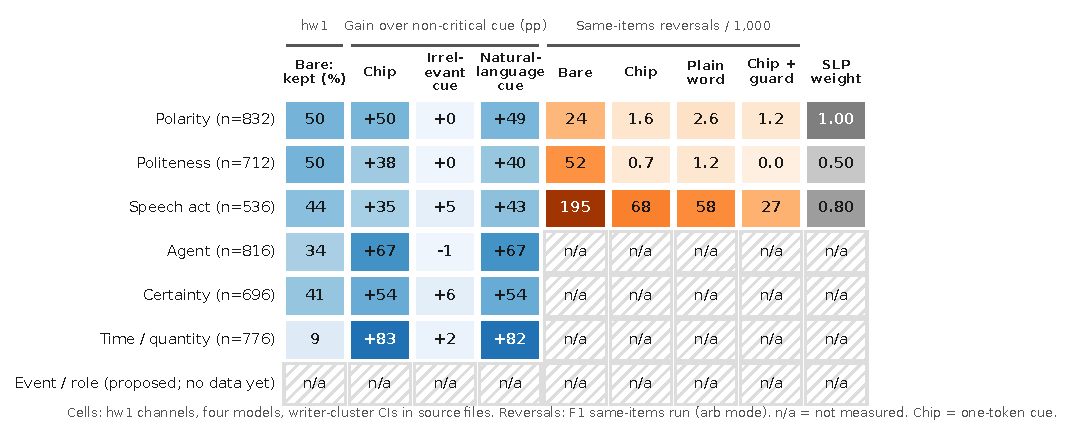
\includegraphics[width=\linewidth]{figs/fig4_dimension_table.pdf}
\caption{Dimension by intervention table. Left: share of bare outputs that keep the critical commitment (hw1, four models), and gain in that share over a non-critical cue for the chip, an irrelevant control cue and a natural-language cue. Right: same-items reversals per 1,000 messages for bare, chip, plain word and chip plus guard (\jmfOneUnits{} units; measured only for polarity, politeness and speech act), and the SLP severity weight (mean of two expert raters, $n=2$). Event/role structure is proposed but has no data. Every cell is printed; shading is redundant. Sources: \texttt{figs/figure\_values.json}.}\label{fig:table}
\Description{Dimension by intervention table.}
\end{figure}

\subsection{Cue Restoration Priced Per 1,000 Messages on the Same Items}\label{sec:price}

\paragraph{Design.}
The gains above come from constructed pairs. To price the cue on the messages that people actually shorten, we returned to the elicitation sample and took the \jmfOneUnits{} units whose source carried a cue that the human keywords dropped (polarity \jmfOneUnitsPol{}, politeness \jmfOneUnitsPolite{}, sentence type \jmfOneUnitsAct{}, the last a seeded subsample of question and request units). Each unit was regenerated by \jmfOneModels{} models (GPT-6.1-terra, Qwen2.5-7B, Llama-3.1-8B) under four arms at temperature zero: the stored bare output, the cue as a chip, the cue as a plain word, and the chip with the guard of \S\ref{sec:guard} monitoring the supplied chip. The restoration share is the proportion of units whose output honours the dropped cue; reversals per 1,000 messages are the exposure per 1,000 messages times one minus the restoration share. The bare arm reproduces the always-commit rates of \S\ref{sec:basecost}, so the unit construction matches. Disputed critical labels (\jmfOneArbRows{} rows) were resolved by the blind arbiter.

\paragraph{Results.}
Table~\ref{tab:price} gives the prices. Giving the cue on every message lowers polarity reversals from \jmfOneRevPolBare{} to \jmfOneRevPolChip{} (chip) or \jmfOneRevPolWord{} (word) per 1,000, and politeness reversals from \jmfOneRevPoliteBare{} to \jmfOneRevPoliteChip{} or \jmfOneRevPoliteWord{}. Chip and word are equivalent within 5 points on politeness (chip minus word \jmfOneChipMinusWordPolite{} points [\jmfOneChipMinusWordPoliteLo{}, \jmfOneChipMinusWordPoliteHi{}]) and not distinguishable on polarity (\jmfOneChipMinusWordPol{} [\jmfOneChipMinusWordPolLo{}, \jmfOneChipMinusWordPolHi{}]) or sentence type (\jmfOneChipMinusWordAct{} [\jmfOneChipMinusWordActLo{}, \jmfOneChipMinusWordActHi{}]). The guard on the chip arm helps on all three (polarity \jmfOneGuardGainPol{} points [\jmfOneGuardGainPolLo{}, \jmfOneGuardGainPolHi{}], politeness \jmfOneGuardGainPolite{} [\jmfOneGuardGainPoliteLo{}, \jmfOneGuardGainPoliteHi{}], sentence type \jmfOneGuardGainAct{} [\jmfOneGuardGainActLo{}, \jmfOneGuardGainActHi{}]); it raises the share of sentence-type units that honour the cue from \jmfOneRestActChip{}\% to \jmfOneRestActChipG{}\% [\jmfOneRestActChipGLo{}, \jmfOneRestActChipGHi{}]. Sentence type keeps the largest residual (\jmfOneRevActChipG{} [\jmfOneRevActChipGLo{}, \jmfOneRevActChipGHi{}] per 1,000 with chip and guard, from \jmfOneRevActBare{} bare), consistent with the speech-act dimension being the hardest in every earlier study.

\begin{table}[t]
\caption{Same-items price of the default and of cue restoration (\jmfOneUnits{} elicitation units, \jmfOneModels{} models, message-bootstrap 95\% intervals, arbiter-resolved labels). Each cell is the share of units whose output honours the dropped cue, followed by reversals per 1,000 messages if the arm is applied to every message and a cue is supplied each time. The price is the best case for the cue arms: it ignores the cost of cueing messages that need no cue and assumes the cue is elicited.}\label{tab:price}
\small
\begin{tabular}{lccccc}
\toprule
Dimension (units) & Quantity & Bare & Chip & Plain word & Chip + guard \\
\midrule
Polarity (\jmfOneUnitsPol{}) & Restored (\%) & \jmfOneRestPolBare{} & \jmfOneRestPolChip{} & \jmfOneRestPolWord{} & \jmfOneRestPolChipG{} \\
 & Reversals /1,000 & \jmfOneRevPolBare{} & \jmfOneRevPolChip{} [\jmfOneRevPolChipLo{}, \jmfOneRevPolChipHi{}] & \jmfOneRevPolWord{} [\jmfOneRevPolWordLo{}, \jmfOneRevPolWordHi{}] & \jmfOneRevPolChipG{} [\jmfOneRevPolChipGLo{}, \jmfOneRevPolChipGHi{}] \\
\addlinespace
Politeness (\jmfOneUnitsPolite{}) & Restored (\%) & \jmfOneRestPoliteBare{} & \jmfOneRestPoliteChip{} & \jmfOneRestPoliteWord{} & \jmfOneRestPoliteChipG{} \\
 & Reversals /1,000 & \jmfOneRevPoliteBare{} & \jmfOneRevPoliteChip{} [\jmfOneRevPoliteChipLo{}, \jmfOneRevPoliteChipHi{}] & \jmfOneRevPoliteWord{} [\jmfOneRevPoliteWordLo{}, \jmfOneRevPoliteWordHi{}] & \jmfOneRevPoliteChipG{} [\jmfOneRevPoliteChipGLo{}, \jmfOneRevPoliteChipGHi{}] \\
\addlinespace
Sentence type (\jmfOneUnitsAct{}) & Restored (\%) & \jmfOneRestActBare{} & \jmfOneRestActChip{} & \jmfOneRestActWord{} & \jmfOneRestActChipG{} \\
 & Reversals /1,000 & \jmfOneRevActBare{} & \jmfOneRevActChip{} [\jmfOneRevActChipLo{}, \jmfOneRevActChipHi{}] & \jmfOneRevActWord{} [\jmfOneRevActWordLo{}, \jmfOneRevActWordHi{}] & \jmfOneRevActChipG{} [\jmfOneRevActChipGLo{}, \jmfOneRevActChipGHi{}] \\
\bottomrule
\end{tabular}
\end{table}

\paragraph{A superseded estimate.}
An earlier version of this price transported the cue-honouring rate from the constructed pairs to the elicitation units. The measured rates do not match the transported ones for polarity or politeness (the transported rate was too optimistic for polarity and too pessimistic for politeness, in each case outside 5 points and outside the interval), so the measured rows replace the transported rows throughout.

\paragraph{Bound.}
Machine-judged outputs, three models, one prompt template, \jmfOneUnitsPol{} polarity units, and a price that assumes the cue is supplied. The restored outputs have no separate human check beyond the arbiter check (Section~\ref{sec:m-arbiter}).

% ------------------------------------------------------------------------------------------------
\subsection{Prior-Work Recap: The Commitment Guard}\label{sec:guard}

This subsection recaps the guard studies reported in our two earlier papers \cite{concurrent_se4all,concurrent_caleai}. It is subordinate to the writer-intent result: nothing in the argument of Section~\ref{sec:s4} depends on it, and the new material here is the human repair-usability audit (Section~\ref{sec:usability}) and the severity weighting (Section~\ref{sec:severity}).

\paragraph{Guard and baselines.}
The guard (G1) is a monitor on the output plus a bounded retry. The monitor flags an output that contradicts a supplied cue or that adds politeness the keywords do not carry; on a flag the model gets one short feedback turn that names the commitment it must keep, up to two retries at temperature zero, stopping at the first output the monitor does not flag. The monitor is a deterministic, rule-based extractor. A guard can look effective for a trivial reason, so we compare it with three alternatives that share the monitor, the trigger and the retry budget: a strip-only arm (G1s) that deletes an unsupplied ``please'' and makes no model call; a resample arm (G1r) that retries from the original prompt with no feedback at temperature $0.7$; and a feedback arm at temperature $0.7$ (G1t) that isolates feedback from decoding. The no-feedback baseline is G1r. The endpoint is a machine-scored partial predicate (the critical commitment and the absence of added politeness), not a usability judgement; usability is the subject of \S\ref{sec:usability}.

\paragraph{Transfer to fresh families (restated from our earlier papers).}
This result and the discovery-set guard result are reported in our earlier papers \cite{concurrent_se4all,concurrent_caleai}; we restate them here once, with the same frozen guard, because the audits below depend on them.
The frozen guard was applied, without change, to \jmgtFamilies{} fresh speech-act families that were not used to design it (\jmgtTargets{} target occurrences, \jmgwFlaggedF{} flagged requests). Joint pass rises from \jmgtJointP{}\% [\jmgtJointPLo{}, \jmgtJointPHi{}] to \jmgtJointG{}\% [\jmgtJointGLo{}, \jmgtJointGHi{}], a gain of \jmgwGain{} points [\jmgwGainLo{}, \jmgwGainHi{}]. Of the \jmgwStrictRepairN{} first-pass strict failures, \jmgwStrictRepairK{} (\jmgwStrictRepair{}\% [\jmgwStrictRepairLo{}, \jmgwStrictRepairHi{}]) are repaired; the guard rewrote \jmgwChangedK{} of \jmgwChangedN{} first-pass-correct targets and turned \jmgwPassToFailK{} passes into failures. The whole run took \jmgwGenCalls{} generation calls. On the discovery set the corresponding joint pass is \jmgbDiscPZero{}\% to \jmgbDiscGOne{}\% [\jmgbDiscGOneLo{}, \jmgbDiscGOneHi{}].

\paragraph{The no-feedback baseline.}
Table~\ref{tab:guard} compares the arms. Resampling without feedback gives about the strip-only gain on the fresh families (\jmgbWcGOner{}\% against \jmgbWcGOnes{}\%) and repairs \jmgbWcRepairGOner{}\% of strict failures against \jmgbWcRepairGOnes{}\% for the strip and \jmgbWcRepairGOne{}\% for the guard. The paired joint-pass contrast of the guard over the resample is \jmgbCWcGOneMGOner{} points [\jmgbCWcGOneMGOnerLo{}, \jmgbCWcGOneMGOnerHi{}] on the fresh families and \jmgbCDiscGOneMGOner{} [\jmgbCDiscGOneMGOnerLo{}, \jmgbCDiscGOneMGOnerHi{}] on the discovery set. Because the resample runs at temperature $0.7$ and the guard at zero, the clean contrast for the value of feedback is G1t minus G1r: \jmgbCWcGOnetMGOner{} points [\jmgbCWcGOnetMGOnerLo{}, \jmgbCWcGOnetMGOnerHi{}] on the fresh families and \jmgbCDiscGOnetMGOner{} [\jmgbCDiscGOnetMGOnerLo{}, \jmgbCDiscGOnetMGOnerHi{}] on discovery. Feedback adds value beyond resampling on both sets, and temperature is not what separates the guard from the baseline (G1 minus G1t: \jmgbCWcGOneMGOnet{} [\jmgbCWcGOneMGOnetLo{}, \jmgbCWcGOneMGOnetHi{}] on fresh families). The guard also beats the strip alone by \jmgwGOneMinusGOnes{} points [\jmgwGOneMinusGOnesLo{}, \jmgwGOneMinusGOnesHi{}], so the deletion explains part of the gain and not all of it.

\begin{table}[t]
\caption{The guard against its baselines (machine-scored joint pass, family-bootstrap 95\% intervals; strict repair is the share of first-pass strict failures repaired). Fresh families: \jmgbWcFamilies{} speech-act families, \jmgbWcTargets{} targets. Discovery: \jmgbDiscFamilies{} families, \jmgbDiscTargets{} targets. G1r is the no-feedback resample at temperature $0.7$.}\label{tab:guard}
\small
\begin{tabular}{lcccc}
\toprule
 & \multicolumn{2}{c}{Fresh families} & \multicolumn{2}{c}{Discovery} \\
\cmidrule(lr){2-3}\cmidrule(lr){4-5}
Arm & Joint pass (\%) & Strict repair & Joint pass (\%) & Strict repair \\
\midrule
First pass (P0) & \jmgbWcPZero{} [\jmgbWcPZeroLo{}, \jmgbWcPZeroHi{}] & --- & \jmgbDiscPZero{} [\jmgbDiscPZeroLo{}, \jmgbDiscPZeroHi{}] & --- \\
Strip only (G1s) & \jmgbWcGOnes{} [\jmgbWcGOnesLo{}, \jmgbWcGOnesHi{}] & \jmgbWcRepairGOnesK{}/\jmgbWcRepairGOnesN{} & \jmgbDiscGOnes{} [\jmgbDiscGOnesLo{}, \jmgbDiscGOnesHi{}] & \jmgbDiscRepairGOnesK{}/\jmgbDiscRepairGOnesN{} \\
Resample, no feedback (G1r) & \jmgbWcGOner{} [\jmgbWcGOnerLo{}, \jmgbWcGOnerHi{}] & \jmgbWcRepairGOnerK{}/\jmgbWcRepairGOnerN{} & \jmgbDiscGOner{} [\jmgbDiscGOnerLo{}, \jmgbDiscGOnerHi{}] & \jmgbDiscRepairGOnerK{}/\jmgbDiscRepairGOnerN{} \\
Feedback at $T=0.7$ (G1t) & \jmgbWcGOnet{} [\jmgbWcGOnetLo{}, \jmgbWcGOnetHi{}] & \jmgbWcRepairGOnetK{}/\jmgbWcRepairGOnetN{} & \jmgbDiscGOnet{} [\jmgbDiscGOnetLo{}, \jmgbDiscGOnetHi{}] & \jmgbDiscRepairGOnetK{}/\jmgbDiscRepairGOnetN{} \\
Guard (G1) & \jmgbWcGOne{} [\jmgbWcGOneLo{}, \jmgbWcGOneHi{}] & \jmgbWcRepairGOneK{}/\jmgbWcRepairGOneN{} & \jmgbDiscGOne{} [\jmgbDiscGOneLo{}, \jmgbDiscGOneHi{}] & \jmgbDiscRepairGOneK{}/\jmgbDiscRepairGOneN{} \\
\bottomrule
\end{tabular}
\end{table}

\paragraph{Bound.}
The endpoint is a machine-scored partial predicate on speech-act families; it supports the claim that the guard repairs commitment violations that a no-feedback retry does not, not a claim that its output is usable, fluent or preferred. Those questions are answered next, by people.

% ------------------------------------------------------------------------------------------------
\subsection{Repair Usability: A Blind Three-Rater Audit}\label{sec:usability}

\paragraph{Design.}
A guard that changes the text can make it worse to read. We audited this with a blind human audit under a decision rule frozen before any rating returned. The audit uses \jmpOneSevenItemsPerArm{} repaired texts and \jmpOneSevenItemsPerArm{} control texts (unrepaired outputs for which the monitor raised no flag, drawn from the same two pools), none of which had appeared in an earlier audit, rated by \jmpOneSevenRaters{} adult non-author classmates, \jmpOneSevenPerItem{} raters per item, with the arm hidden. The primary endpoint is the item-level majority of ``usable as the person's message''; secondary endpoints are meaning preserved against the keywords and cues and an invented stance or attitude. The frozen rule reads: if the interval for repaired minus control usable lies wholly below $-10$ points, the guard fails as a deployment clause; if it includes $-10$ but excludes zero, report a cost of uncertain size; if it includes zero, report no detectable cost. A comparison arm was added before any return to address the fact that controls never failed and repaired items did: the first-pass output that the guard replaced (\jmpOneSevenOrigItems{} items, each paired with its repair).

\paragraph{Result under the frozen rule.}
Repaired texts were usable in \jmpOneSevenRepUsableK{} of \jmpOneSevenRepUsableN{} items (\jmpOneSevenRepUsable{}\% [\jmpOneSevenRepUsableLo{}, \jmpOneSevenRepUsableHi{}]) and control texts in \jmpOneSevenCtlUsableK{} of \jmpOneSevenCtlUsableN{} (\jmpOneSevenCtlUsable{}\% [\jmpOneSevenCtlUsableLo{}, \jmpOneSevenCtlUsableHi{}]). The difference is \jmpOneSevenDiffUsable{} points [\jmpOneSevenDiffUsableLo{}, \jmpOneSevenDiffUsableHi{}]. The interval includes zero, so under the frozen rule the audit detects no usability cost, but the interval extends to \jmpOneSevenDiffUsableLo{} points: the audit is inconclusive, it neither shows nor excludes a cost, and it does not establish equivalence. Table~\ref{tab:p17} gives the endpoints. Repaired texts preserved the meaning less often than controls (\jmpOneSevenDiffPres{} points [\jmpOneSevenDiffPresLo{}, \jmpOneSevenDiffPresHi{}]) and so did the combined endpoint, usable and preserving (\jmpOneSevenDiffUsPres{} [\jmpOneSevenDiffUsPresLo{}, \jmpOneSevenDiffUsPresHi{}]); invented stance did not differ (\jmpOneSevenDiffStance{} [\jmpOneSevenDiffStanceLo{}, \jmpOneSevenDiffStanceHi{}]). The comparison is between inputs the first pass got wrong and inputs it got right, so the gap partly measures item difficulty and not the repair; the comparison against each repair's own failed original, below, holds the item fixed.

\begin{table}[t]
\caption{Blind audit of guard repairs (the repair-usability audit; \jmpOneSevenRaters{} raters, \jmpOneSevenPerItem{} per item, item-level strict majority; Wilson 95\% intervals for rates, Newcombe 95\% intervals for differences; preserving and stance exclude one item with no majority). The items are a pre-specified deterministic list, not a probability sample, so the rates describe these items.}\label{tab:p17}
\small
\begin{tabular}{lccc}
\toprule
Endpoint & Repaired & Control & Repaired $-$ control (points) \\
\midrule
Usable (primary) & \jmpOneSevenRepUsableK{}/\jmpOneSevenRepUsableN{} = \jmpOneSevenRepUsable{}\% [\jmpOneSevenRepUsableLo{}, \jmpOneSevenRepUsableHi{}] & \jmpOneSevenCtlUsableK{}/\jmpOneSevenCtlUsableN{} = \jmpOneSevenCtlUsable{}\% [\jmpOneSevenCtlUsableLo{}, \jmpOneSevenCtlUsableHi{}] & \jmpOneSevenDiffUsable{} [\jmpOneSevenDiffUsableLo{}, \jmpOneSevenDiffUsableHi{}] \\
Meaning preserved & \jmpOneSevenRepPresK{}/\jmpOneSevenRepPresN{} = \jmpOneSevenRepPres{}\% [\jmpOneSevenRepPresLo{}, \jmpOneSevenRepPresHi{}] & \jmpOneSevenCtlPresK{}/\jmpOneSevenCtlPresN{} = \jmpOneSevenCtlPres{}\% [\jmpOneSevenCtlPresLo{}, \jmpOneSevenCtlPresHi{}] & \jmpOneSevenDiffPres{} [\jmpOneSevenDiffPresLo{}, \jmpOneSevenDiffPresHi{}] \\
Invented stance & \jmpOneSevenRepStanceK{}/\jmpOneSevenRepStanceN{} = \jmpOneSevenRepStance{}\% [\jmpOneSevenRepStanceLo{}, \jmpOneSevenRepStanceHi{}] & \jmpOneSevenCtlStanceK{}/\jmpOneSevenCtlStanceN{} = \jmpOneSevenCtlStance{}\% [\jmpOneSevenCtlStanceLo{}, \jmpOneSevenCtlStanceHi{}] & \jmpOneSevenDiffStance{} [\jmpOneSevenDiffStanceLo{}, \jmpOneSevenDiffStanceHi{}] \\
\bottomrule
\end{tabular}
\end{table}

\paragraph{Against each repair's own failed original.}
Paired with the first-pass output that the guard replaced, repairs preserve the meaning more often (\jmpOneSevenOrigPres{} points [\jmpOneSevenOrigPresLo{}, \jmpOneSevenOrigPresHi{}], $p=\jmpOneSevenOrigPresP{}$ on \jmpOneSevenOrigPresPairs{} pairs) and invent a stance less often (\jmpOneSevenOrigStance{} points [\jmpOneSevenOrigStanceLo{}, \jmpOneSevenOrigStanceHi{}], $p=\jmpOneSevenOrigStanceP{}$ on \jmpOneSevenOrigStancePairs{} pairs). Usability shows no detectable change (\jmpOneSevenOrigUsable{} points [\jmpOneSevenOrigUsableLo{}, \jmpOneSevenOrigUsableHi{}], $p=\jmpOneSevenOrigUsableP{}$). Relative to the failed original, the repair preserves the meaning and removes the invented stance without a detectable change in how usable the sentence is.

\paragraph{Heterogeneity.}
Usability varies by the model that produced the repair. Gemma-3-4B repairs are usable in \jmpOneSevenRepGemmaUsableK{} of \jmpOneSevenRepGemmaUsableN{} (\jmpOneSevenRepGemmaUsable{}\%), against \jmpOneSevenRepLlamaUsableK{} of \jmpOneSevenRepLlamaUsableN{} for Llama-3.1-8B, \jmpOneSevenRepQwenSUsableK{} of \jmpOneSevenRepQwenSUsableN{} for Qwen2.5-7B and \jmpOneSevenRepTerraUsableK{} of \jmpOneSevenRepTerraUsableN{} for GPT-6.1-terra. These are descriptive counts on an unbalanced list. They suggest that a repair is only as readable as the repairing model's prose, which the pooled estimate hides.

\paragraph{Bound.}
\jmpOneSevenItemsPerArm{} items per arm from a fixed list, classmate raters rather than AAC users or clinicians, and a rule that detects no cost without excluding a cost of up to \jmpOneSevenDiffUsableLo{} points.

% ------------------------------------------------------------------------------------------------
\subsection{Weighting the Failures by Clinical Severity}\label{sec:severity}

Two speech-language pathologists, anonymous and paid as expert annotators of study materials, rated how serious each kind of silent meaning change would be if spoken as a client's message, and then rated stored outputs with the arm hidden: guard repairs (\jmslpAccRepairN{} ratings), the matching first-pass originals (\jmslpAccOrigN{}), chip outputs (\jmslpAccChipN{}) and plain-word outputs (\jmslpAccWordN{}); a rating is one rater's judgement of one output. This is an expert review with $n=2$ raters, not a population estimate, and the agreement statistics describe these two raters. Both rated negation dropped or added as the most serious change (\jmslpNegSeverity{} of 5) and both would block it (\jmslpNegBlock{}\%).

We weight each judge-flagged failure by the severity of its type, taking the largest weight on an output. On the fresh speech-act families the guard lowers the weighted failure rate from \jmslpWGuardBase{}\% to \jmslpWGuardG{}\% (strip only: \jmslpWGuardGs{}\%; unweighted \jmslpUGuardBase{}\% to \jmslpUGuardG{}\%; \jmslpWcN{} targets). On the human-written pairs the weighted failure rate is \jmslpWCueBare{}\% for bare keywords, \jmslpWCueChip{}\% with a chip and \jmslpWCueWord{}\% with a plain word, against \jmslpWCueIrrel{}\% with an irrelevant chip (\jmslpHwN{} rows per arm). The bare and irrelevant rates are inflated by the pair design, because two variants share one bare input; the comparison of interest is chip against word against the irrelevant control, and it again shows that the cue content carries the effect.

Rated directly, the SLPs judged the guard's repairs acceptable to speak as they stand in \jmslpAccRepair{}\% of ratings, and as they stand or after a small edit in \jmslpRepairEdit{}\%, against \jmslpAccOrig{}\% as they stand for the matching originals. Chip outputs were acceptable as they stand in \jmslpAccChip{}\% of ratings and plain-word outputs in \jmslpAccWord{}\%. The two raters agreed on whether an output says what the selected words mean on \jmslpAgreeA{}\% of items ($\kappa=\jmslpKappaA{}$) and on whether it is acceptable to speak on \jmslpAgreeB{}\% ($\kappa=\jmslpKappaB{}$); we report these as descriptions of this pair. The arms were rated on different numbers of items, so the acceptability figures are descriptive and do not rank the arms.

% ------------------------------------------------------------------------------------------------
\subsection{What These Studies Establish}\label{sec:establish}

The default is measurable, mostly attributable to a missing cue, and a supplied cue removes most of it on the dimensions measured. Against people's own keyword choices the affirmative default is the right guess for negation and costs about \jmtTwoRevPol{} silent reversals per 1,000 messages; it is not a prompt artefact and holds in \jmbreadthModels{} models from \jmbreadthFamilies{} families; a one-token cue or a plain word removes nearly all of the negation and politeness cost on the same items (to \jmfOneRevPolChip{} and \jmfOneRevPoliteChip{} per 1,000 with a chip); the cue's content, not its presence, does the work; and the guard (recapped in Section~\ref{sec:guard}) repairs violations that a no-feedback retry does not, and the blind repair audit could not exclude a usability cost (Section~\ref{sec:usability}). These results answer whether a commitment is preserved. Whether the preserved draft is the message the writer meant is a different question, which \S\ref{sec:waterfall} takes up with the writers themselves.
.
% Every number is a \jm... macro from make_macros.py (function s3() and earlier functions); no hand-typed numbers.
% Examples are stored outputs chosen by a declared rule (analysis/hw1/examples.md). Citations are limited to
% records already in refs.bib; nothing new was opened for this section.
% Labels defined here: sec:default (section), sec:basecost, sec:robust, sec:cue, sec:price, sec:asks, sec:guard, sec:usability, sec:severity.
% Needs \usepackage{booktabs} (acmart loads it).

\section{Studies and Results I: Defaults, Cue Restoration and the Guard}\label{sec:default}

This section reports the studies that establish what the default costs and what repairs it. Each study states its population, its estimator and its denominator, and each result is bounded once, where it is reported. We begin with the cost of the default measured against what people actually type (\S\ref{sec:basecost}), test whether the default belongs to the prompt or to the models (\S\ref{sec:robust}), show that a cue restores the commitment and that the cue's content is what does it (\S\ref{sec:cue}), price the restoration per 1,000 messages on the same items (\S\ref{sec:price}), ask whether any rule for when to ask beats chance (\S\ref{sec:asks}), and then evaluate the guard against a no-feedback baseline (\S\ref{sec:guard}), a blind human audit of its repairs (\S\ref{sec:usability}) and expert severity weights (\S\ref{sec:severity}).

\paragraph{Conventions common to all studies.}
Model outputs are labelled by two machine judges (J1, J2); disagreements on the critical commitment go to a blind arbiter that sees only the output text, and no label falls back to J1 when the arbiter is missing. Intervals are 95\% percentile bootstrap intervals clustered by writer (human-written pairs), by family (machine-written families and the guard) or by message (the elicitation sample). The human-written, legend, control and guard analyses use \jmconvBoot{} resamples with seed \jmconvSeed{}, the same-items study uses \jmconvBootFOne{} resamples with seed \jmconvSeedFOne{}, and the elicitation-sample prices and ask-policy contrasts use the resample counts stated in their reports. Rates ``per 1,000 messages'' are rates over the sampled units, not deployment rates. Where a decision rule governs a verdict (the legend test, the same-items comparisons, the guard baseline and the usability audit), it was written down and git-timestamped before the outcomes it governs were generated or returned; we do not call any of the studies pre-registered. Machine labels are used throughout this section; where a human check of the machine labels exists it is reported in the study that uses the labels, and the checks that have not yet returned are named as such.

% ------------------------------------------------------------------------------------------------
\subsection{What the Default Costs, Priced Against Human Base Rates}\label{sec:basecost}

\paragraph{Setting.}
A keyword string that omits a cue leaves the model to choose a reading, and the choice is a default. Whether a default is a good guess depends on how often the omitted cue was present in what the writer meant. We measured that base rate from people. The elicitation sample consists of \jmtTwoMessages{} source messages from an AAC-style corpus (\jmtTwoCorpus{} messages in total, of which \jmtTwoCorpusNeg{}\% are negated by a detector label), each shortened to keywords by three human keyword sets, giving \jmtTwoUnits{} keyword units. Stored outputs of \jmbreadthOrigModels{} generators were scored for three commitment dimensions (negation, politeness, sentence type), the dimensions for which a lexical test of ``the keywords carry the cue'' exists. The source cue labels are detector labels; these labels have no human check, so the prices below carry the detector's error and are provisional.

\paragraph{Affirmative is the right guess for negation; the cost is the asymmetry.}
Among keyword strings with no negation word, the source was negated in \jmtTwoPostPol{}\% [\jmtTwoPostPolLo{}, \jmtTwoPostPolHi{}] of cases (\jmtTwoPostBayesPol{}\% by Bayes' rule with the corpus prevalence; \jmtTwoPolRandHalf{}\% in the unweighted random half). Guessing the affirmative reading is therefore correct for all but a few messages in a hundred, and the models take it: they output an affirmative sentence for \jmtTwoAffGivenNoNeg{}\% of such inputs. The direction of the default is the rational one, which is consistent with prior reports that language models state negative content too positively \cite{chen2023say}; we do not present the default as new. What the base rate adds is the price. People dropped the negation word from \jmtTwoDroppedPol{}\% [\jmtTwoDroppedPolLo{}, \jmtTwoDroppedPolHi{}] of the negated messages, so an affirmative sentence silently reverses \jmtTwoRevPol{} [\jmtTwoRevPolLo{}, \jmtTwoRevPolHi{}] messages per 1,000, while a spurious negation is introduced in \jmtTwoSpurPol{} per 1,000. The affirmative guess breaks even with the opposite guess only if a reversed negation costs less than \jmtTwoBreakPol{} times a spurious one, and a prompt would have to be shown on about \jmtTwoQueriesPol{} inputs per reversal it prevents. The models' confidence also exceeds the evidence: they assert a negation on \jmtTwoModelCuePol{}\% of these inputs where the base rate is \jmtTwoPostPol{}\%.

\paragraph{Politeness and sentence type differ in kind.}
For politeness the default is calibrated: the source was polite in \jmtTwoPostPolite{}\% [\jmtTwoPostPoliteLo{}, \jmtTwoPostPoliteHi{}] of unmarked inputs and models add politeness to \jmtTwoModelCuePolite{}\%. Politeness the writer typed is lost for \jmtTwoRevPolite{} messages per 1,000, with a break-even ratio of \jmtTwoBreakPolite{}, so the asymmetry is milder than for negation; the opposite error, politeness added to a plain message, occurs in \jmtTwoSpurPolite{} per 1,000. For sentence type the statement default is not the Bayes-preferred guess at all: the source was a question, request or other non-statement in \jmtTwoPostAct{}\% [\jmtTwoPostActLo{}, \jmtTwoPostActHi{}] of unmarked inputs, while models assert one on only \jmtTwoModelCueAct{}\%, and \jmtTwoRevAct{} [\jmtTwoRevActLo{}, \jmtTwoRevActHi{}] messages per 1,000 have their sentence type reversed or flattened (break-even ratio \jmtTwoBreakAct{}: the statement default pays only if the two errors cost about the same).
Table~\ref{tab:basecost} collects these rows.

\begin{table}[t]
\caption{The default priced against human base rates (elicitation sample, \jmtTwoUnits{} keyword units from \jmtTwoMessages{} messages; Horvitz--Thompson weights; message-bootstrap 95\% intervals). Prior is the share of keyword strings without the cue whose source message carried it; model asserts cue is the share of such inputs for which the model's output asserts the cue-bearing value. Reversals are messages whose source has the cue, whose keywords lack it and whose output lacks it; the opposite error is an output that asserts the cue when the source lacks it; break-even is the cost ratio of a reversal to an opposite error at which the default stops paying. Source labels are detector labels.}\label{tab:basecost}
\footnotesize
\begin{tabular}{@{}lccccc@{}}
\toprule
Dimension & Prior [95\% CI] & Model asserts cue & Reversals /1,000 [CI] & Opposite /1,000 & Break-even \\
\midrule
Negation (affirmative default) & \jmtTwoPostPol{}\% [\jmtTwoPostPolLo{}, \jmtTwoPostPolHi{}] & \jmtTwoModelCuePol{}\% & \jmtTwoRevPol{} [\jmtTwoRevPolLo{}, \jmtTwoRevPolHi{}] & \jmtTwoSpurPol{} & \jmtTwoBreakPol{} \\
Politeness (plain default) & \jmtTwoPostPolite{}\% [\jmtTwoPostPoliteLo{}, \jmtTwoPostPoliteHi{}] & \jmtTwoModelCuePolite{}\% & \jmtTwoRevPolite{} [\jmtTwoRevPoliteLo{}, \jmtTwoRevPoliteHi{}] & \jmtTwoSpurPolite{} & \jmtTwoBreakPolite{} \\
Sentence type (statement default) & \jmtTwoPostAct{}\% [\jmtTwoPostActLo{}, \jmtTwoPostActHi{}] & \jmtTwoModelCueAct{}\% & \jmtTwoRevAct{} [\jmtTwoRevActLo{}, \jmtTwoRevActHi{}] & \jmtTwoSpurAct{} & \jmtTwoBreakAct{} \\
\bottomrule
\end{tabular}
\end{table}

\paragraph{The same default in human-written pairs.}
The human-written pairs (\S\ref{sec:cue}) test the default where the truth is known. Each pair differs in one commitment and shares one bare input, so a model that commits to one reading is wrong on exactly one variant and the true affirmative rate is 50\%. On the bare channel the models chose the affirmative reading in \jmtTwoHwAffShare{}\% of valid outputs.

\paragraph{Bound.}
Source cue labels are detector labels, the sentence-type ``no cue'' condition is a lexical proxy, the frame prevalence of negation (\jmtTwoPrevPol{}\%) exceeds the corpus value, and the prices are rates over a sampled elicitation frame. We therefore read the table as the cost structure of the default, not as a deployment rate.

% ------------------------------------------------------------------------------------------------
\paragraph{Appendix material.} The model-breadth tables and legend test (Appendix~\ref{sec:robust}) and the ask-policy arithmetic (Appendix~\ref{sec:asks}) are in the appendix; the main text uses only their headline results.

\subsection{A Cue Restores the Commitment, and the Content of the Cue Does It}\label{sec:cue}

\paragraph{Human-written pairs.}
To move beyond machine-written test items, \jmhwWritersTotal{} adult non-author classmates wrote sentence pairs that differ in one commitment and chose their own keywords; pairs were kept only after classmate checks, and \jmhwFamilies{} families were analysed, with \jmhwChipGainWriters{} to \jmhwAffShareWriters{} writers contributing to each contrast. Each family was expanded by \jmbreadthOrigModels{} models under bare keywords, a non-critical extra keyword, the cue as a one-token chip (for example \texttt{[NOT]}), the full cue set, and the full original text. The primary contrasts are those of the machine-written confirmation set (Holm-corrected over three); the human-written pairs are an exploratory replication of them. The chip gain over a non-critical word on speech act is \jmhwChipGain{} points [\jmhwChipGainLo{}, \jmhwChipGainHi{}] (\jmhwChipGainWriters{} writers, \jmhwChipGainFamilies{} families). When the full sentence is given, politeness is added to plain messages more often than it is removed from polite ones, by \jmhwPolGain{} points [\jmhwPolGainLo{}, \jmhwPolGainHi{}]. The bare affirmative share (\jmhwAffAll{}\%, \S\ref{sec:basecost}) is the third contrast. All three agree in direction and in decision with the machine-written confirmation set. Because each contrast rests on a handful of writers, we claim the direction and its consistency across writers and models, not the width of the intervals.

\paragraph{One stored case, by declared rule.}
The rule: order the analysed polarity families by the SHA-256 of the family identifier and take the first one in which a bare output commits to the wrong value while the chip output matches. That family is \texttt{hw-pol-075}, the model is Gemma-3-4B, and the target is the negated reading of ``The supervisor does not read my schedule.''

\begin{center}\small
\begin{tabular}{lll}
\toprule
Channel & Input & Stored output \\
\midrule
bare & \texttt{supervisor read} & ``The supervisor read.'' (affirmative) \\
chip & \texttt{[NOT] supervisor read} & ``The supervisor did not read.'' (negated) \\
\bottomrule
\end{tabular}
\end{center}

\noindent
In this dimension a bare output commits to the wrong value in \jmexPolBareWrong{}\% [\jmexPolBareWrongLo{}, \jmexPolBareWrongHi{}] of bare rows (the design ceiling), and when it does the chip output matches the target in \jmexPolRepair{}\% [\jmexPolRepairLo{}, \jmexPolRepairHi{}] of \jmexPolRepairN{} such rows. The same rule applied to speech act selects a family whose chip outputs match the target in a smaller share, \jmexActRepair{}\% [\jmexActRepairLo{}, \jmexActRepairHi{}] of \jmexActRepairN{} rows, in line with the larger residual for sentence type in \S\ref{sec:price}.

\paragraph{Six dimensions.}
Table~\ref{tab:sixdim} reports the cue gain for every measured dimension with its two controls. An irrelevant chip (a cue from another dimension, with the same token cost) adds about nothing on polarity, politeness, agent and time (at most \jmctlIrrelAddTime{} points) and a small amount on certainty (\jmctlIrrelAddCert{} [\jmctlIrrelAddCertLo{}, \jmctlIrrelAddCertHi{}]) and speech act (\jmctlIrrelAddAct{} [\jmctlIrrelAddActLo{}, \jmctlIrrelAddActHi{}]). The relevant chip beats the irrelevant chip by \jmctlOverIrrelAct{} to \jmctlOverIrrelTime{} points, so the gain is the content of the cue and not the presence of an extra token. A plain-language word delivers the same restoration as the chip within 5 points on every dimension except speech act; on speech act the word is better than the chip (chip minus word \jmctlOverWordAct{} points [\jmctlOverWordActLo{}, \jmctlOverWordActHi{}]). We do not claim that the chip is better than a plain word.

\begin{table}[t]
\caption{Cue restoration and its controls in human-written pairs (critical-commitment match, pooled over four models, writer-cluster 95\% intervals; points). Chip gain is chip minus non-critical word. Polarity and politeness bare matches sit at 50\% by design because both variants share one bare input; their informative quantity is the gain. Full input is the whole original sentence.}\label{tab:sixdim}
\small
\begin{tabular}{lccccc}
\toprule
Dimension & Bare match (\%) & Chip match (\%) & Chip gain [CI] & Irrelevant chip adds [CI] & Chip $-$ word [CI] \\
\midrule
Agent & \jmhwMatchBareAgent{} & \jmhwMatchChipAgent{} & \jmctlGAgent{} [\jmctlGAgentLo{}, \jmctlGAgentHi{}] & \jmctlIrrelAddAgent{} [\jmctlIrrelAddAgentLo{}, \jmctlIrrelAddAgentHi{}] & \jmctlOverWordAgent{} [\jmctlOverWordAgentLo{}, \jmctlOverWordAgentHi{}] \\
Time / quantity & \jmhwMatchBareTime{} & \jmhwMatchChipTime{} & \jmctlGTime{} [\jmctlGTimeLo{}, \jmctlGTimeHi{}] & \jmctlIrrelAddTime{} [\jmctlIrrelAddTimeLo{}, \jmctlIrrelAddTimeHi{}] & \jmctlOverWordTime{} [\jmctlOverWordTimeLo{}, \jmctlOverWordTimeHi{}] \\
Certainty & \jmhwMatchBareCert{} & \jmhwMatchChipCert{} & \jmctlGCert{} [\jmctlGCertLo{}, \jmctlGCertHi{}] & \jmctlIrrelAddCert{} [\jmctlIrrelAddCertLo{}, \jmctlIrrelAddCertHi{}] & \jmctlOverWordCert{} [\jmctlOverWordCertLo{}, \jmctlOverWordCertHi{}] \\
Polarity & \jmhwMatchBarePol{} & \jmhwMatchChipPol{} & \jmctlGPol{} [\jmctlGPolLo{}, \jmctlGPolHi{}] & \jmctlIrrelAddPol{} [\jmctlIrrelAddPolLo{}, \jmctlIrrelAddPolHi{}] & \jmctlOverWordPol{} [\jmctlOverWordPolLo{}, \jmctlOverWordPolHi{}] \\
Politeness & \jmhwMatchBarePolite{} & \jmhwMatchChipPolite{} & \jmctlGPolite{} [\jmctlGPoliteLo{}, \jmctlGPoliteHi{}] & \jmctlIrrelAddPolite{} [\jmctlIrrelAddPoliteLo{}, \jmctlIrrelAddPoliteHi{}] & \jmctlOverWordPolite{} [\jmctlOverWordPoliteLo{}, \jmctlOverWordPoliteHi{}] \\
Speech act & \jmhwMatchBareAct{} & \jmhwMatchChipAct{} & \jmctlGAct{} [\jmctlGActLo{}, \jmctlGActHi{}] & \jmctlIrrelAddAct{} [\jmctlIrrelAddActLo{}, \jmctlIrrelAddActHi{}] & \jmctlOverWordAct{} [\jmctlOverWordActLo{}, \jmctlOverWordActHi{}] \\
\bottomrule
\end{tabular}
\end{table}

\paragraph{Bound.}
\jmhwChipGainWriters{} to \jmhwAffShareWriters{} writers per dimension, one prompt template, and machine labels (with a blind arbiter for disputes); treated outputs have no separate human check beyond the arbiter check (Section~\ref{sec:m-arbiter}).

% ------------------------------------------------------------------------------------------------

\begin{figure}[t]
\centering
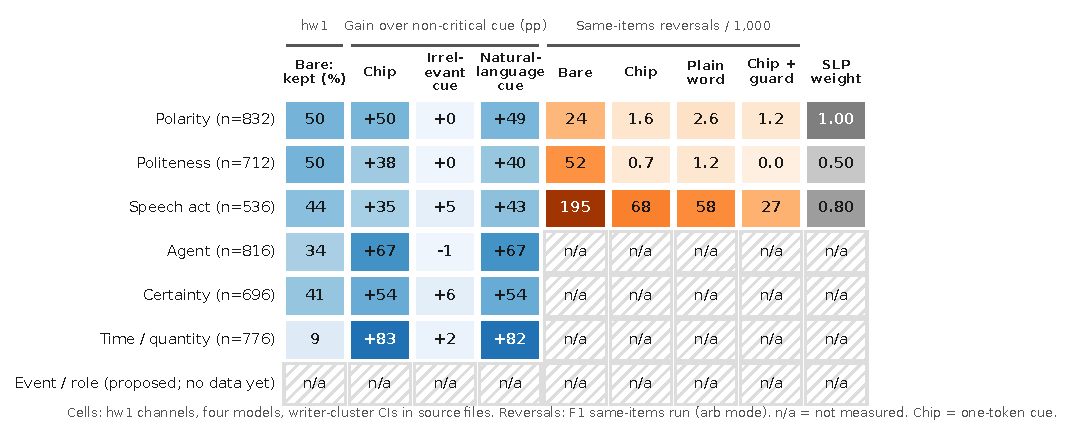
\includegraphics[width=\linewidth]{figs/fig4_dimension_table.pdf}
\caption{Dimension by intervention table. Left: share of bare outputs that keep the critical commitment (hw1, four models), and gain in that share over a non-critical cue for the chip, an irrelevant control cue and a natural-language cue. Right: same-items reversals per 1,000 messages for bare, chip, plain word and chip plus guard (\jmfOneUnits{} units; measured only for polarity, politeness and speech act), and the SLP severity weight (mean of two expert raters, $n=2$). Event/role structure is proposed but has no data. Every cell is printed; shading is redundant. Sources: \texttt{figs/figure\_values.json}.}\label{fig:table}
\Description{Dimension by intervention table.}
\end{figure}

\subsection{Cue Restoration Priced Per 1,000 Messages on the Same Items}\label{sec:price}

\paragraph{Design.}
The gains above come from constructed pairs. To price the cue on the messages that people actually shorten, we returned to the elicitation sample and took the \jmfOneUnits{} units whose source carried a cue that the human keywords dropped (polarity \jmfOneUnitsPol{}, politeness \jmfOneUnitsPolite{}, sentence type \jmfOneUnitsAct{}, the last a seeded subsample of question and request units). Each unit was regenerated by \jmfOneModels{} models (GPT-6.1-terra, Qwen2.5-7B, Llama-3.1-8B) under four arms at temperature zero: the stored bare output, the cue as a chip, the cue as a plain word, and the chip with the guard of \S\ref{sec:guard} monitoring the supplied chip. The restoration share is the proportion of units whose output honours the dropped cue; reversals per 1,000 messages are the exposure per 1,000 messages times one minus the restoration share. The bare arm reproduces the always-commit rates of \S\ref{sec:basecost}, so the unit construction matches. Disputed critical labels (\jmfOneArbRows{} rows) were resolved by the blind arbiter.

\paragraph{Results.}
Table~\ref{tab:price} gives the prices. Giving the cue on every message lowers polarity reversals from \jmfOneRevPolBare{} to \jmfOneRevPolChip{} (chip) or \jmfOneRevPolWord{} (word) per 1,000, and politeness reversals from \jmfOneRevPoliteBare{} to \jmfOneRevPoliteChip{} or \jmfOneRevPoliteWord{}. Chip and word are equivalent within 5 points on politeness (chip minus word \jmfOneChipMinusWordPolite{} points [\jmfOneChipMinusWordPoliteLo{}, \jmfOneChipMinusWordPoliteHi{}]) and not distinguishable on polarity (\jmfOneChipMinusWordPol{} [\jmfOneChipMinusWordPolLo{}, \jmfOneChipMinusWordPolHi{}]) or sentence type (\jmfOneChipMinusWordAct{} [\jmfOneChipMinusWordActLo{}, \jmfOneChipMinusWordActHi{}]). The guard on the chip arm helps on all three (polarity \jmfOneGuardGainPol{} points [\jmfOneGuardGainPolLo{}, \jmfOneGuardGainPolHi{}], politeness \jmfOneGuardGainPolite{} [\jmfOneGuardGainPoliteLo{}, \jmfOneGuardGainPoliteHi{}], sentence type \jmfOneGuardGainAct{} [\jmfOneGuardGainActLo{}, \jmfOneGuardGainActHi{}]); it raises the share of sentence-type units that honour the cue from \jmfOneRestActChip{}\% to \jmfOneRestActChipG{}\% [\jmfOneRestActChipGLo{}, \jmfOneRestActChipGHi{}]. Sentence type keeps the largest residual (\jmfOneRevActChipG{} [\jmfOneRevActChipGLo{}, \jmfOneRevActChipGHi{}] per 1,000 with chip and guard, from \jmfOneRevActBare{} bare), consistent with the speech-act dimension being the hardest in every earlier study.

\begin{table}[t]
\caption{Same-items price of the default and of cue restoration (\jmfOneUnits{} elicitation units, \jmfOneModels{} models, message-bootstrap 95\% intervals, arbiter-resolved labels). Each cell is the share of units whose output honours the dropped cue, followed by reversals per 1,000 messages if the arm is applied to every message and a cue is supplied each time. The price is the best case for the cue arms: it ignores the cost of cueing messages that need no cue and assumes the cue is elicited.}\label{tab:price}
\small
\begin{tabular}{lccccc}
\toprule
Dimension (units) & Quantity & Bare & Chip & Plain word & Chip + guard \\
\midrule
Polarity (\jmfOneUnitsPol{}) & Restored (\%) & \jmfOneRestPolBare{} & \jmfOneRestPolChip{} & \jmfOneRestPolWord{} & \jmfOneRestPolChipG{} \\
 & Reversals /1,000 & \jmfOneRevPolBare{} & \jmfOneRevPolChip{} [\jmfOneRevPolChipLo{}, \jmfOneRevPolChipHi{}] & \jmfOneRevPolWord{} [\jmfOneRevPolWordLo{}, \jmfOneRevPolWordHi{}] & \jmfOneRevPolChipG{} [\jmfOneRevPolChipGLo{}, \jmfOneRevPolChipGHi{}] \\
\addlinespace
Politeness (\jmfOneUnitsPolite{}) & Restored (\%) & \jmfOneRestPoliteBare{} & \jmfOneRestPoliteChip{} & \jmfOneRestPoliteWord{} & \jmfOneRestPoliteChipG{} \\
 & Reversals /1,000 & \jmfOneRevPoliteBare{} & \jmfOneRevPoliteChip{} [\jmfOneRevPoliteChipLo{}, \jmfOneRevPoliteChipHi{}] & \jmfOneRevPoliteWord{} [\jmfOneRevPoliteWordLo{}, \jmfOneRevPoliteWordHi{}] & \jmfOneRevPoliteChipG{} [\jmfOneRevPoliteChipGLo{}, \jmfOneRevPoliteChipGHi{}] \\
\addlinespace
Sentence type (\jmfOneUnitsAct{}) & Restored (\%) & \jmfOneRestActBare{} & \jmfOneRestActChip{} & \jmfOneRestActWord{} & \jmfOneRestActChipG{} \\
 & Reversals /1,000 & \jmfOneRevActBare{} & \jmfOneRevActChip{} [\jmfOneRevActChipLo{}, \jmfOneRevActChipHi{}] & \jmfOneRevActWord{} [\jmfOneRevActWordLo{}, \jmfOneRevActWordHi{}] & \jmfOneRevActChipG{} [\jmfOneRevActChipGLo{}, \jmfOneRevActChipGHi{}] \\
\bottomrule
\end{tabular}
\end{table}

\paragraph{A superseded estimate.}
An earlier version of this price transported the cue-honouring rate from the constructed pairs to the elicitation units. The measured rates do not match the transported ones for polarity or politeness (the transported rate was too optimistic for polarity and too pessimistic for politeness, in each case outside 5 points and outside the interval), so the measured rows replace the transported rows throughout.

\paragraph{Bound.}
Machine-judged outputs, three models, one prompt template, \jmfOneUnitsPol{} polarity units, and a price that assumes the cue is supplied. The restored outputs have no separate human check beyond the arbiter check (Section~\ref{sec:m-arbiter}).

% ------------------------------------------------------------------------------------------------
\subsection{Prior-Work Recap: The Commitment Guard}\label{sec:guard}

This subsection recaps the guard studies reported in our two earlier papers \cite{concurrent_se4all,concurrent_caleai}. It is subordinate to the writer-intent result: nothing in the argument of Section~\ref{sec:s4} depends on it, and the new material here is the human repair-usability audit (Section~\ref{sec:usability}) and the severity weighting (Section~\ref{sec:severity}).

\paragraph{Guard and baselines.}
The guard (G1) is a monitor on the output plus a bounded retry. The monitor flags an output that contradicts a supplied cue or that adds politeness the keywords do not carry; on a flag the model gets one short feedback turn that names the commitment it must keep, up to two retries at temperature zero, stopping at the first output the monitor does not flag. The monitor is a deterministic, rule-based extractor. A guard can look effective for a trivial reason, so we compare it with three alternatives that share the monitor, the trigger and the retry budget: a strip-only arm (G1s) that deletes an unsupplied ``please'' and makes no model call; a resample arm (G1r) that retries from the original prompt with no feedback at temperature $0.7$; and a feedback arm at temperature $0.7$ (G1t) that isolates feedback from decoding. The no-feedback baseline is G1r. The endpoint is a machine-scored partial predicate (the critical commitment and the absence of added politeness), not a usability judgement; usability is the subject of \S\ref{sec:usability}.

\paragraph{Transfer to fresh families (restated from our earlier papers).}
This result and the discovery-set guard result are reported in our earlier papers \cite{concurrent_se4all,concurrent_caleai}; we restate them here once, with the same frozen guard, because the audits below depend on them.
The frozen guard was applied, without change, to \jmgtFamilies{} fresh speech-act families that were not used to design it (\jmgtTargets{} target occurrences, \jmgwFlaggedF{} flagged requests). Joint pass rises from \jmgtJointP{}\% [\jmgtJointPLo{}, \jmgtJointPHi{}] to \jmgtJointG{}\% [\jmgtJointGLo{}, \jmgtJointGHi{}], a gain of \jmgwGain{} points [\jmgwGainLo{}, \jmgwGainHi{}]. Of the \jmgwStrictRepairN{} first-pass strict failures, \jmgwStrictRepairK{} (\jmgwStrictRepair{}\% [\jmgwStrictRepairLo{}, \jmgwStrictRepairHi{}]) are repaired; the guard rewrote \jmgwChangedK{} of \jmgwChangedN{} first-pass-correct targets and turned \jmgwPassToFailK{} passes into failures. The whole run took \jmgwGenCalls{} generation calls. On the discovery set the corresponding joint pass is \jmgbDiscPZero{}\% to \jmgbDiscGOne{}\% [\jmgbDiscGOneLo{}, \jmgbDiscGOneHi{}].

\paragraph{The no-feedback baseline.}
Table~\ref{tab:guard} compares the arms. Resampling without feedback gives about the strip-only gain on the fresh families (\jmgbWcGOner{}\% against \jmgbWcGOnes{}\%) and repairs \jmgbWcRepairGOner{}\% of strict failures against \jmgbWcRepairGOnes{}\% for the strip and \jmgbWcRepairGOne{}\% for the guard. The paired joint-pass contrast of the guard over the resample is \jmgbCWcGOneMGOner{} points [\jmgbCWcGOneMGOnerLo{}, \jmgbCWcGOneMGOnerHi{}] on the fresh families and \jmgbCDiscGOneMGOner{} [\jmgbCDiscGOneMGOnerLo{}, \jmgbCDiscGOneMGOnerHi{}] on the discovery set. Because the resample runs at temperature $0.7$ and the guard at zero, the clean contrast for the value of feedback is G1t minus G1r: \jmgbCWcGOnetMGOner{} points [\jmgbCWcGOnetMGOnerLo{}, \jmgbCWcGOnetMGOnerHi{}] on the fresh families and \jmgbCDiscGOnetMGOner{} [\jmgbCDiscGOnetMGOnerLo{}, \jmgbCDiscGOnetMGOnerHi{}] on discovery. Feedback adds value beyond resampling on both sets, and temperature is not what separates the guard from the baseline (G1 minus G1t: \jmgbCWcGOneMGOnet{} [\jmgbCWcGOneMGOnetLo{}, \jmgbCWcGOneMGOnetHi{}] on fresh families). The guard also beats the strip alone by \jmgwGOneMinusGOnes{} points [\jmgwGOneMinusGOnesLo{}, \jmgwGOneMinusGOnesHi{}], so the deletion explains part of the gain and not all of it.

\begin{table}[t]
\caption{The guard against its baselines (machine-scored joint pass, family-bootstrap 95\% intervals; strict repair is the share of first-pass strict failures repaired). Fresh families: \jmgbWcFamilies{} speech-act families, \jmgbWcTargets{} targets. Discovery: \jmgbDiscFamilies{} families, \jmgbDiscTargets{} targets. G1r is the no-feedback resample at temperature $0.7$.}\label{tab:guard}
\small
\begin{tabular}{lcccc}
\toprule
 & \multicolumn{2}{c}{Fresh families} & \multicolumn{2}{c}{Discovery} \\
\cmidrule(lr){2-3}\cmidrule(lr){4-5}
Arm & Joint pass (\%) & Strict repair & Joint pass (\%) & Strict repair \\
\midrule
First pass (P0) & \jmgbWcPZero{} [\jmgbWcPZeroLo{}, \jmgbWcPZeroHi{}] & --- & \jmgbDiscPZero{} [\jmgbDiscPZeroLo{}, \jmgbDiscPZeroHi{}] & --- \\
Strip only (G1s) & \jmgbWcGOnes{} [\jmgbWcGOnesLo{}, \jmgbWcGOnesHi{}] & \jmgbWcRepairGOnesK{}/\jmgbWcRepairGOnesN{} & \jmgbDiscGOnes{} [\jmgbDiscGOnesLo{}, \jmgbDiscGOnesHi{}] & \jmgbDiscRepairGOnesK{}/\jmgbDiscRepairGOnesN{} \\
Resample, no feedback (G1r) & \jmgbWcGOner{} [\jmgbWcGOnerLo{}, \jmgbWcGOnerHi{}] & \jmgbWcRepairGOnerK{}/\jmgbWcRepairGOnerN{} & \jmgbDiscGOner{} [\jmgbDiscGOnerLo{}, \jmgbDiscGOnerHi{}] & \jmgbDiscRepairGOnerK{}/\jmgbDiscRepairGOnerN{} \\
Feedback at $T=0.7$ (G1t) & \jmgbWcGOnet{} [\jmgbWcGOnetLo{}, \jmgbWcGOnetHi{}] & \jmgbWcRepairGOnetK{}/\jmgbWcRepairGOnetN{} & \jmgbDiscGOnet{} [\jmgbDiscGOnetLo{}, \jmgbDiscGOnetHi{}] & \jmgbDiscRepairGOnetK{}/\jmgbDiscRepairGOnetN{} \\
Guard (G1) & \jmgbWcGOne{} [\jmgbWcGOneLo{}, \jmgbWcGOneHi{}] & \jmgbWcRepairGOneK{}/\jmgbWcRepairGOneN{} & \jmgbDiscGOne{} [\jmgbDiscGOneLo{}, \jmgbDiscGOneHi{}] & \jmgbDiscRepairGOneK{}/\jmgbDiscRepairGOneN{} \\
\bottomrule
\end{tabular}
\end{table}

\paragraph{Bound.}
The endpoint is a machine-scored partial predicate on speech-act families; it supports the claim that the guard repairs commitment violations that a no-feedback retry does not, not a claim that its output is usable, fluent or preferred. Those questions are answered next, by people.

% ------------------------------------------------------------------------------------------------
\subsection{Repair Usability: A Blind Three-Rater Audit}\label{sec:usability}

\paragraph{Design.}
A guard that changes the text can make it worse to read. We audited this with a blind human audit under a decision rule frozen before any rating returned. The audit uses \jmpOneSevenItemsPerArm{} repaired texts and \jmpOneSevenItemsPerArm{} control texts (unrepaired outputs for which the monitor raised no flag, drawn from the same two pools), none of which had appeared in an earlier audit, rated by \jmpOneSevenRaters{} adult non-author classmates, \jmpOneSevenPerItem{} raters per item, with the arm hidden. The primary endpoint is the item-level majority of ``usable as the person's message''; secondary endpoints are meaning preserved against the keywords and cues and an invented stance or attitude. The frozen rule reads: if the interval for repaired minus control usable lies wholly below $-10$ points, the guard fails as a deployment clause; if it includes $-10$ but excludes zero, report a cost of uncertain size; if it includes zero, report no detectable cost. A comparison arm was added before any return to address the fact that controls never failed and repaired items did: the first-pass output that the guard replaced (\jmpOneSevenOrigItems{} items, each paired with its repair).

\paragraph{Result under the frozen rule.}
Repaired texts were usable in \jmpOneSevenRepUsableK{} of \jmpOneSevenRepUsableN{} items (\jmpOneSevenRepUsable{}\% [\jmpOneSevenRepUsableLo{}, \jmpOneSevenRepUsableHi{}]) and control texts in \jmpOneSevenCtlUsableK{} of \jmpOneSevenCtlUsableN{} (\jmpOneSevenCtlUsable{}\% [\jmpOneSevenCtlUsableLo{}, \jmpOneSevenCtlUsableHi{}]). The difference is \jmpOneSevenDiffUsable{} points [\jmpOneSevenDiffUsableLo{}, \jmpOneSevenDiffUsableHi{}]. The interval includes zero, so under the frozen rule the audit detects no usability cost, but the interval extends to \jmpOneSevenDiffUsableLo{} points: the audit is inconclusive, it neither shows nor excludes a cost, and it does not establish equivalence. Table~\ref{tab:p17} gives the endpoints. Repaired texts preserved the meaning less often than controls (\jmpOneSevenDiffPres{} points [\jmpOneSevenDiffPresLo{}, \jmpOneSevenDiffPresHi{}]) and so did the combined endpoint, usable and preserving (\jmpOneSevenDiffUsPres{} [\jmpOneSevenDiffUsPresLo{}, \jmpOneSevenDiffUsPresHi{}]); invented stance did not differ (\jmpOneSevenDiffStance{} [\jmpOneSevenDiffStanceLo{}, \jmpOneSevenDiffStanceHi{}]). The comparison is between inputs the first pass got wrong and inputs it got right, so the gap partly measures item difficulty and not the repair; the comparison against each repair's own failed original, below, holds the item fixed.

\begin{table}[t]
\caption{Blind audit of guard repairs (the repair-usability audit; \jmpOneSevenRaters{} raters, \jmpOneSevenPerItem{} per item, item-level strict majority; Wilson 95\% intervals for rates, Newcombe 95\% intervals for differences; preserving and stance exclude one item with no majority). The items are a pre-specified deterministic list, not a probability sample, so the rates describe these items.}\label{tab:p17}
\small
\begin{tabular}{lccc}
\toprule
Endpoint & Repaired & Control & Repaired $-$ control (points) \\
\midrule
Usable (primary) & \jmpOneSevenRepUsableK{}/\jmpOneSevenRepUsableN{} = \jmpOneSevenRepUsable{}\% [\jmpOneSevenRepUsableLo{}, \jmpOneSevenRepUsableHi{}] & \jmpOneSevenCtlUsableK{}/\jmpOneSevenCtlUsableN{} = \jmpOneSevenCtlUsable{}\% [\jmpOneSevenCtlUsableLo{}, \jmpOneSevenCtlUsableHi{}] & \jmpOneSevenDiffUsable{} [\jmpOneSevenDiffUsableLo{}, \jmpOneSevenDiffUsableHi{}] \\
Meaning preserved & \jmpOneSevenRepPresK{}/\jmpOneSevenRepPresN{} = \jmpOneSevenRepPres{}\% [\jmpOneSevenRepPresLo{}, \jmpOneSevenRepPresHi{}] & \jmpOneSevenCtlPresK{}/\jmpOneSevenCtlPresN{} = \jmpOneSevenCtlPres{}\% [\jmpOneSevenCtlPresLo{}, \jmpOneSevenCtlPresHi{}] & \jmpOneSevenDiffPres{} [\jmpOneSevenDiffPresLo{}, \jmpOneSevenDiffPresHi{}] \\
Invented stance & \jmpOneSevenRepStanceK{}/\jmpOneSevenRepStanceN{} = \jmpOneSevenRepStance{}\% [\jmpOneSevenRepStanceLo{}, \jmpOneSevenRepStanceHi{}] & \jmpOneSevenCtlStanceK{}/\jmpOneSevenCtlStanceN{} = \jmpOneSevenCtlStance{}\% [\jmpOneSevenCtlStanceLo{}, \jmpOneSevenCtlStanceHi{}] & \jmpOneSevenDiffStance{} [\jmpOneSevenDiffStanceLo{}, \jmpOneSevenDiffStanceHi{}] \\
\bottomrule
\end{tabular}
\end{table}

\paragraph{Against each repair's own failed original.}
Paired with the first-pass output that the guard replaced, repairs preserve the meaning more often (\jmpOneSevenOrigPres{} points [\jmpOneSevenOrigPresLo{}, \jmpOneSevenOrigPresHi{}], $p=\jmpOneSevenOrigPresP{}$ on \jmpOneSevenOrigPresPairs{} pairs) and invent a stance less often (\jmpOneSevenOrigStance{} points [\jmpOneSevenOrigStanceLo{}, \jmpOneSevenOrigStanceHi{}], $p=\jmpOneSevenOrigStanceP{}$ on \jmpOneSevenOrigStancePairs{} pairs). Usability shows no detectable change (\jmpOneSevenOrigUsable{} points [\jmpOneSevenOrigUsableLo{}, \jmpOneSevenOrigUsableHi{}], $p=\jmpOneSevenOrigUsableP{}$). Relative to the failed original, the repair preserves the meaning and removes the invented stance without a detectable change in how usable the sentence is.

\paragraph{Heterogeneity.}
Usability varies by the model that produced the repair. Gemma-3-4B repairs are usable in \jmpOneSevenRepGemmaUsableK{} of \jmpOneSevenRepGemmaUsableN{} (\jmpOneSevenRepGemmaUsable{}\%), against \jmpOneSevenRepLlamaUsableK{} of \jmpOneSevenRepLlamaUsableN{} for Llama-3.1-8B, \jmpOneSevenRepQwenSUsableK{} of \jmpOneSevenRepQwenSUsableN{} for Qwen2.5-7B and \jmpOneSevenRepTerraUsableK{} of \jmpOneSevenRepTerraUsableN{} for GPT-6.1-terra. These are descriptive counts on an unbalanced list. They suggest that a repair is only as readable as the repairing model's prose, which the pooled estimate hides.

\paragraph{Bound.}
\jmpOneSevenItemsPerArm{} items per arm from a fixed list, classmate raters rather than AAC users or clinicians, and a rule that detects no cost without excluding a cost of up to \jmpOneSevenDiffUsableLo{} points.

% ------------------------------------------------------------------------------------------------
\subsection{Weighting the Failures by Clinical Severity}\label{sec:severity}

Two speech-language pathologists, anonymous and paid as expert annotators of study materials, rated how serious each kind of silent meaning change would be if spoken as a client's message, and then rated stored outputs with the arm hidden: guard repairs (\jmslpAccRepairN{} ratings), the matching first-pass originals (\jmslpAccOrigN{}), chip outputs (\jmslpAccChipN{}) and plain-word outputs (\jmslpAccWordN{}); a rating is one rater's judgement of one output. This is an expert review with $n=2$ raters, not a population estimate, and the agreement statistics describe these two raters. Both rated negation dropped or added as the most serious change (\jmslpNegSeverity{} of 5) and both would block it (\jmslpNegBlock{}\%).

We weight each judge-flagged failure by the severity of its type, taking the largest weight on an output. On the fresh speech-act families the guard lowers the weighted failure rate from \jmslpWGuardBase{}\% to \jmslpWGuardG{}\% (strip only: \jmslpWGuardGs{}\%; unweighted \jmslpUGuardBase{}\% to \jmslpUGuardG{}\%; \jmslpWcN{} targets). On the human-written pairs the weighted failure rate is \jmslpWCueBare{}\% for bare keywords, \jmslpWCueChip{}\% with a chip and \jmslpWCueWord{}\% with a plain word, against \jmslpWCueIrrel{}\% with an irrelevant chip (\jmslpHwN{} rows per arm). The bare and irrelevant rates are inflated by the pair design, because two variants share one bare input; the comparison of interest is chip against word against the irrelevant control, and it again shows that the cue content carries the effect.

Rated directly, the SLPs judged the guard's repairs acceptable to speak as they stand in \jmslpAccRepair{}\% of ratings, and as they stand or after a small edit in \jmslpRepairEdit{}\%, against \jmslpAccOrig{}\% as they stand for the matching originals. Chip outputs were acceptable as they stand in \jmslpAccChip{}\% of ratings and plain-word outputs in \jmslpAccWord{}\%. The two raters agreed on whether an output says what the selected words mean on \jmslpAgreeA{}\% of items ($\kappa=\jmslpKappaA{}$) and on whether it is acceptable to speak on \jmslpAgreeB{}\% ($\kappa=\jmslpKappaB{}$); we report these as descriptions of this pair. The arms were rated on different numbers of items, so the acceptability figures are descriptive and do not rank the arms.

% ------------------------------------------------------------------------------------------------
\subsection{What These Studies Establish}\label{sec:establish}

The default is measurable, mostly attributable to a missing cue, and a supplied cue removes most of it on the dimensions measured. Against people's own keyword choices the affirmative default is the right guess for negation and costs about \jmtTwoRevPol{} silent reversals per 1,000 messages; it is not a prompt artefact and holds in \jmbreadthModels{} models from \jmbreadthFamilies{} families; a one-token cue or a plain word removes nearly all of the negation and politeness cost on the same items (to \jmfOneRevPolChip{} and \jmfOneRevPoliteChip{} per 1,000 with a chip); the cue's content, not its presence, does the work; and the guard (recapped in Section~\ref{sec:guard}) repairs violations that a no-feedback retry does not, and the blind repair audit could not exclude a usability cost (Section~\ref{sec:usability}). These results answer whether a commitment is preserved. Whether the preserved draft is the message the writer meant is a different question, which \S\ref{sec:waterfall} takes up with the writers themselves.
